
\usetikzlibrary{arrows, chains, positioning}

\tikzset{
defaultNode1/.style={rectangle, draw, minimum height=8mm, minimum width=2mm, node distance=0mm},
defaultNode2/.style={defaultNode1, minimum width=0mm},
greyNode/.style={fill=lightgray},
secondNode/.style={on chain},
}

%Erster Innerer Knoten einer Ebene.
%\param #1 : 1. Referenzschlüsseleintrag
%\param #2 : 2. Referenzschlüsseleintrag
%\param #3 : 3. Referenzschlüsseleintrag
%\param #4 : 4. Referenzschlüsseleintrag
%\param #5 : Ebene auf der sich der Knoten befindet
%\param #6 : Name des Knotens (am besten fortlaufende Zahlen verwenden)
%\param #7 : Offset in x-Richtung
\tikzset{pics/firstInnerNode/.style n args={7}{
code={
	\node[defaultNode, greyNode](#6+0) at (#7,-#5*2) {};
	\chainin (#6+0);
	\node[defaultNode, secondNode]{#1};
	\node[defaultNode, secondNode, greyNode](#6+1){};
	\node[defaultNode, secondNode]{#2};
	\node[defaultNode, secondNode, greyNode](#6+2){};
	\node[defaultNode, secondNode]{#3};
	\node[defaultNode, secondNode, greyNode](#6+3){};
	\node[defaultNode, secondNode]{#4};
	\node[defaultNode, secondNode, greyNode](#6+4){};
}}}

%Innerer Knoten.
%\param #1 : 1. Referenzschlüsseleintrag
%\param #2 : 2. Referenzschlüsseleintrag
%\param #3 : 3. Referenzschlüsseleintrag
%\param #4 : 4. Referenzschlüsseleintrag
%\param #5 : Ebene auf der sich der Knoten befindet
%\param #6 : Name des Knotens (am besten fortlaufende Zahlen verwenden)
\tikzset{pics/innerNode/.style n args={6}{
code={

	\node[defaultNode,node distance=12mm, secondNode, greyNode](#6+0){};
	\node[defaultNode, secondNode]{#1};
	\node[defaultNode, secondNode, greyNode](#6+1){};
	\node[defaultNode, secondNode]{#2};
	\node[defaultNode, secondNode, greyNode](#6+2){};
	\node[defaultNode, secondNode]{#3};
	\node[defaultNode, secondNode, greyNode](#6+3){};
	\node[defaultNode, secondNode]{#4};
	\node[defaultNode, secondNode, greyNode](#6+4){};
}}}

%Innerer Knoten, variable Distanz.
%\param #1 : 1. Referenzschlüsseleintrag
%\param #2 : 2. Referenzschlüsseleintrag
%\param #3 : 3. Referenzschlüsseleintrag
%\param #4 : 4. Referenzschlüsseleintrag
%\param #5 : Ebene auf der sich der Knoten befindet
%\param #6 : Name des Knotens (am besten fortlaufende Zahlen verwenden)
\tikzset{pics/innerNodeVar/.style n args={7}{
code={
	\node[defaultNode,node distance=#7, secondNode, greyNode](#6+0){};
	\node[defaultNode, secondNode]{#1};
	\node[defaultNode, secondNode, greyNode](#6+1){};
	\node[defaultNode, secondNode]{#2};
	\node[defaultNode, secondNode, greyNode](#6+2){};
	\node[defaultNode, secondNode]{#3};
	\node[defaultNode, secondNode, greyNode](#6+3){};
	\node[defaultNode, secondNode]{#4};
	\node[defaultNode, secondNode, greyNode](#6+4){};
}}}

%Innerer Knoten, weniger Abstand.
%\param #1 : 1. Referenzschlüsseleintrag
%\param #2 : 2. Referenzschlüsseleintrag
%\param #3 : 3. Referenzschlüsseleintrag
%\param #4 : 4. Referenzschlüsseleintrag
%\param #5 : Ebene auf der sich der Knoten befindet
%\param #6 : Name des Knotens (am besten fortlaufende Zahlen verwenden)
\tikzset{pics/innerNodeNarrow/.style n args={6}{
code={
	\node[defaultNode,node distance=3mm, secondNode, greyNode](#6+0){};
	\node[defaultNode, secondNode]{#1};
	\node[defaultNode, secondNode, greyNode](#6+1){};
	\node[defaultNode, secondNode]{#2};
	\node[defaultNode, secondNode, greyNode](#6+2){};
	\node[defaultNode, secondNode]{#3};
	\node[defaultNode, secondNode, greyNode](#6+3){};
	\node[defaultNode, secondNode]{#4};
	\node[defaultNode, secondNode, greyNode](#6+4){};
}}}

%Erster Blattknoten einer Ebene.
%\param #1 : 1. Referenzschlüsseleintrag
%\param #2 : 1. Nutzdateneintrag
%\param #3 : 2. Referenzschlüsseleintrag
%\param #4 : 2. Nutzdateneintrag
%\param #5 : Ebene auf der sich der Knoten befindet
%\param #6 : Name des Knotens (am besten fortlaufende Zahlen verwenden)
%\param #7 : Offset in x-Richtung
\tikzset{pics/firstLeafNode/.style n args={7}{
code={
	\node[defaultNode](#6+0) at (#7,-#5*2) {#1};
	\chainin (#6+0);
	\node[defaultNode, secondNode]{#2};
	\node[defaultNode, secondNode]{#3};
	\node[defaultNode, secondNode]{#4};
}}}

%Blattknoten.
%\param #1 : 1. Referenzschlüsseleintrag
%\param #2 : 1. Nutzdateneintrag
%\param #3 : 2. Referenzschlüsseleintrag
%\param #4 : 2. Nutzdateneintrag
%\param #5 : Ebene auf der sich der Knoten befindet
%\param #6 : Name des Knotens (am besten fortlaufende Zahlen verwenden)
\tikzset{pics/leafNode/.style n args={6}{
code={
	\node[defaultNode,node distance=3.5mm, secondNode](#6+0){#1};
	\node[defaultNode, secondNode]{#2};
	\node[defaultNode, secondNode]{#3};
	\node[defaultNode, secondNode]{#4};
}}}

%Verbindungspfeil zeichnen
%\param #1 : Name des Vaterblocks
%\param #2 : Index des Pointers (beginnend bei 0)
%\param #3 : Name des Kindblocks
\tikzset{pics/connect/.style n args={3}{
code={
	\draw[->] (#1+#2.south) -- (#3+0.north);
}}}


\begin{document}
\title{Übungsblatt~5}
\subtitle{Schlüssel -- B-Baum, B*-Baum}
\maketitle

\begin{note}
Für einige der Übungen des Blattes kann \url{http://faui6g.informatik.uni-erlangen.de/} verwendet werden.
\end{note}

\section*{Lernziele}
\begin{itemize}
	\item Ziele des Schlüsselzugriffs
	\item Hashing als Methode des Schlüsselzugriffs
	\item Wahl der Hashfunktion und Überlaufbehandlung beim Hashing
	\item Lineares Hashing
\end{itemize}


\begin{normalText}
\section*{Literatur}
\HaerderNintyNine{7.4, 7.5, 7.6}

\ElmasriSeventh{16.8}
\end{normalText}

\section{Fragen zur Vorlesung}
\begin{enumerate}[a)]
	\item Wozu dient der Datenbankpuffer?

	\begin{solution}
	Der Datenbankpuffer dient dem Zwischenspeichern von Daten im Hauptspeicher. Ziel ist es, die Performance zu erhöhen, indem man Blöcke nicht erst von der langsamen Platte lesen muss, sondern sie im schnellen Hauptspeicher vorhält.
	\end{solution}


	\item Warum verwendet man nicht einfach die Pufferverwaltung des Betriebssystems?

	\begin{solution}
	\begin{itemize}
		\item Tut man ja. Die Pufferverwaltung des BS ist weiterhin aktiv und kann Daten auf die Platte auslagern, von denen das DBMS glaubt, sie seien im Speicher.

		\item Das Betriebssystem weiß weniger über die anwendungsspezifischen Zugriffsmuster und kann daher keine optimale Strategie anwenden. Für unseren speziellen Anwendungsfall können wir es besser. Das ist der Hauptgrund, warum man sich nicht alleine auf das BS verlässt. Außerdem bietet das Betriebsystem nicht die Schnittstellen, die für die anderen Schichten gebraucht werden (z.\,B. Transaktionssystem).

		\begin{note}
		\item Weitere Überlegung (technisch, müssen die Teilnehmer nicht wissen): Die Pufferverwaltung des BS stellt jedem Programm einen (virtuellen) Adressraum zur Verfügung, den dieses nutzen kann. Es kann dann Seiten dieses virtuellen Adressraumes an beliebige Stellen des physischen Adressraumes schieben oder sie gar auf die Platte auslagern. Die Anwendung sieht davon nichts, sie greift einfach auf Adressen im virtuellen Adressraum zu. In unserem Fall hieße das, wir würden die gesamte Datenbank in den virtuellen Adressraum kopieren und das BS entscheiden lassen, welche Frames/Seiten davon wirklich im Hauptspeicher liegen. Dank \texttt{mmap()} o.\,ä. geht das sogar schnell. Allerdings ist bei 32-bit-Architekturen der Adressraum auf 4\,GiB beschränkt, das ist viel zu wenig. Unter 64-bit Linux stehen pro
Prozess 128\,TiB virtueller Adressraum zur Verfügung, unter 64-bit Windows 8\,TiB. Auch das kann von großen Datenbanken überschritten werden. Man muss also entscheiden, welche Frames im virtuellen Adressraum liegen sollen. Und das ist bereits wieder eine eigene Pufferverwaltung.
		\end{note}
	\end{itemize}
	\end{solution}


	\item Welche Probleme kann ein Puffer im Fehlerfall (z.\,B. Stromausfall) verursachen? Wie kann man damit umgehen?

	\begin{solution}
	Wenn nicht gespeicherte Änderungen im Puffer liegen, gehen sie verloren. Das ist nicht zu ändern und immer unangenehm, besonders aber wenn Inkonsistenzen auftreten.

	Beispiele:
	\begin{itemize}
		\item Änderungen in verzweigten Strukturen (Listen Element verschieben, B-Baum-Splitt): Nachfolger sind schon persistiert, Vorgänger noch nicht $\rightarrow$ es fehlt die Verzweigung, der Nachfolger kann nicht gefunden werden.
		\item Freispeicherverwaltung (vgl. Übung 4 -- Sätze): Ein Satz wurde in einen Block eingefügt, die Freispeichertabelle ist noch nicht angepasst.
		\item Wir überweisen Geld. Abbuchung ist schon auf der Platte, Gutschrift noch nicht $\rightarrow$ Geldvernichtung
	\end{itemize}
	Minimalziel ist es daher immer, einen konsistenten Zustand zu gewährleisten. Ab da können die Anwendungen ihre Arbeit ggf. noch mal machen. Das schafft man z.B. indem man alte Blöcke nicht überschreibt, sondern den neuen Inhalt in neue Blöcke schreibt und atomar umschaltet.

	Bei den ersten beiden Beispielen, weiß das DBMS, welche Änderungen zusammengehören und wieder zu einem konsistenten Zustand führen. Im dritten Beispiel weiß das nur die Anwendung $\rightarrow$ Transaktionen, siehe später
	\end{solution}


	\item Was ist der Unterschied zwischen direkter und indirekter Seitenzuordnung? Was ist der Unterschied zwischen direkter und indirekter Seiteneinbringung?

	\begin{solution}

	\paragraph{Block, Seite und Kachel}
	Zunächst unterscheiden wir die Begriffe Block, Seite und Kachel:
	\begin{description}
		\item[Block] Block auf der physischen Festplatte, es werden immer ganze Blöcke gelesen und geschrieben und von der Platte in den Hauptspeicher transportiert und umgekehrt.
		\item[Kachel] Eine Kachel ist der Platz für einen Block im Datenbankpuffer. %% im (virtuellen) Hauptspeicher
		\item[Seite] Eine Seite ist die Adressierungseinheit an der Pufferschnittstelle. Eine Seite wird auf Blöcke abgebildet und ist genauso groß wie ein Block. Die höhere Softwareschicht arbeitet nur noch mit Seiten.
	\end{description}


	\paragraph{Seitenzuordnung}
	\begin{description}
		\item[Direkte Seitenzuordnung] bedeutet, dass aufeinanderfolgende Seiten auch in aufeinanderfolgenden Blöcken einer Datei abgelegt werden. Man muss sich also nur die erste Blocknummer für ein Segment merken und kann die Blocknummern für alle Seiten des Segments ausrechnen.

		Das hat nichts mit den Kacheln im Puffer zu tun. Im Puffer können die Seiten deshalb trotzdem komplett verstreut liegen und auch einzeln verdrängt werden. Der Puffer merkt sich zu jeder Kachel, welche Seite darin liegt und kann durch die Seitenzuordnung ermitteln, in welchen Block sie geschrieben werden muss.

		\item[Indirekte Seitenzuordnung] heißt, dass über eine Tabelle festgelegt wird, welche Seite auf welchen Block einer Datei abgebildet wird. Hintereinanderliegende Seiten müssen also nicht mehr in aufeinanderfolgenden Blöcken liegen.
	\end{description}

	Direkt ist schneller und benötigt weniger Verwaltungsdaten, dafür ist es aber auch unflexibler.

	\paragraph{Einbringstrategie}
	Die grundlegende Idee ist, dass speichern auf der Festplatte beim Verdrängen aus dem Puffer nicht notwendigerweise sofort ein Einbringen in den Datenbestand sein muss.

	\begin{description}
		\item[Direkte Seiteneinbringung] heißt, dass Seiten, die auf die Platte gespeichert werden, weil sie aus dem Puffer verdrängt werden, sofort in den Datenbestand eingebracht werden. Das heißt, alle Zeiger und Zuordnungstabellen zeigen sofort auf die neuen Daten. Das geschieht im allgemeinen einfach dadurch, dass die Seite wieder in den Block geschrieben wird, aus dem sie gelesen wurde.
		\item[Indirekte Seiteneinbringung] heißt, geänderte Seiten werden nicht sofort, wenn sie aufgrund der Verdrängung aus dem Puffer auf die Platte gespeichert werden, in den Datenbestand eingebracht. Dies geschieht erst später, z.B. nach einer Datenänderung erst dann, wenn alle Daten der Transaktion geändert sind und auch die Seiten der zugehörigen Indexstrukturen (z.B. B-Bäume) angepasst sind. Hierzu werden die verdrängten Seiten zunächst in neue Blöcke geschrieben und diese erst später durch Änderung von Verwaltungsstrukturen als zum Datenbestand gehörig gekennzeichnet.
	\end{description}

Indirekte Seiteneinbringung ist aufwändiger, bietet aber den Vorteil, dass man den alten Block im Fehlerfall wiederherstellen kann, da er ja noch existiert.
 Direkte Seiteneinbringung hingegen ist von sich aus nicht fehlertolerant. Fehlertoleranz kann z.\,B. über das Führen eines Logs erreicht werden. Die Wiederherstellung muss im Fehlerfall dann das Log auswerten und Änderungen rückgängig machen.

Die Kombination indirekter Seiteneinbringung mit direkter Seitenzuordnung wird beispielsweise durch das Twin-Slot-Verfahren (siehe VL-Folie~\TwinSlot) realisiert.
\end{solution}
\end{enumerate}


\beamertxt{\pagebreak}
\section{Eigenschaften von B-Bäumen}
Begründen Sie, warum der folgende Baum kein B-Baum ist.

\begin{center}
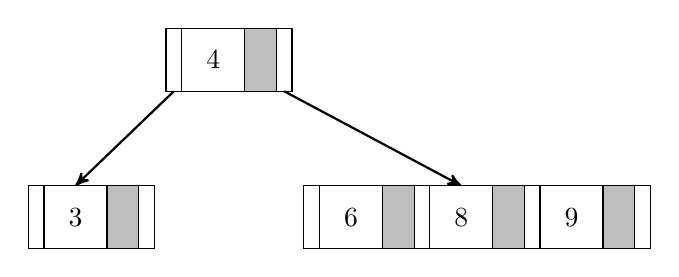
\begin{tikzpicture}
	%arrows
	\draw[thick, ->, >=stealth'] (1.85, 2) -- (0.6,0.8);
	\draw[thick, ->, >=stealth'] (3.25, 2) -- (5.5,0.8);
	%1st lvl
	\node at (2.35, 2.4) {4};

	\fill[fill=lightgray]
		(2.75, 2) rectangle+(0.4, 0.8);

	\draw (1.75,2) rectangle +(1.6, 0.8);

	\draw (1.95, 2) -- (1.95, 2.8)
 		(2.75, 2) -- (2.75, 2.8)
		(3.15, 2) -- (3.15, 2.8);
	%2nd lvl
	\node at (0.6, 0.4) {3};
	\node at (4.1, 0.4) {6};
	\node at (5.5, 0.4) {8};
	\node at (6.9, 0.4) {9};

	\fill[fill=lightgray]
		(1, 0) rectangle+(0.4, 0.8)
		(4.5, 0) rectangle+(0.4, 0.8)
		(5.9, 0) rectangle+(0.4, 0.8)
		(7.3, 0) rectangle+(0.4, 0.8);

	\draw (0,0) rectangle +(1.6,0.8)
		(3.5,0) rectangle +(4.4, 0.8);

	\draw (0.2, 0) -- (0.2, 0.8)
 		(1, 0) -- (1, 0.8)
		(1.4, 0) -- (1.4, 0.8)
 		(3.7, 0) -- (3.7, 0.8)
 		(4.5, 0) -- (4.5, 0.8)
		(4.9, 0) -- (4.9, 0.8)
		 (5.1, 0) -- (5.1, 0.8)
		 (5.9, 0) -- (5.9, 0.8)
		(6.3, 0) -- (6.3, 0.8)
		(6.5, 0) -- (6.5, 0.8)
		(7.3, 0) -- (7.3, 0.8)
		(7.7, 0) -- (7.7, 0.8);
\end{tikzpicture}
\end{center}

\begin{solution}
Es gilt: Jeder Knoten muss mindestens $k$ und darf höchstens $2k$ Einträge haben (außer dem Wurzelknoten). Für $k=1$ ist der linke Blattknoten konform, aber der rechte nicht. Für $k=2$ hingegen ist der rechte Blattknoten zulässig, aber der linke nicht. Daraus folgt, dass der angegebene Baum kein B-Baum ist.
\end{solution}




\section{Einfügen und Löschen im B-Baum}

\begin{enumerate}[a)]
	\item Fügen Sie in einen anfangs leeren B-Baum mit $k=2$ die Zahlen eins bis zwanzig in aufsteigender Reihenfolge ein. Was fällt Ihnen dabei auf?

\begin{solution}
Die Zahlen 1 bis 4 lassen sich problemlos in den Wurzelknoten einfügen.
\begin{center}
    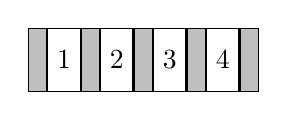
\begin{tikzpicture}[
            start chain=0 going right,
            defaultNode/.style={defaultNode1},
        ]

        %Level0
		\draw pic {firstInnerNode={1}{2}{3}{4}{0}{0}{2}};
    \end{tikzpicture}
\end{center}

Bei 5 kommt es zum Wurzelsplitt und der Baum wächst um eins. Danach steht 3 in der Wurzel, 1 und 2 im linken Blattknoten und 4 und 5 im rechten Blattknoten.

\begin{center}
    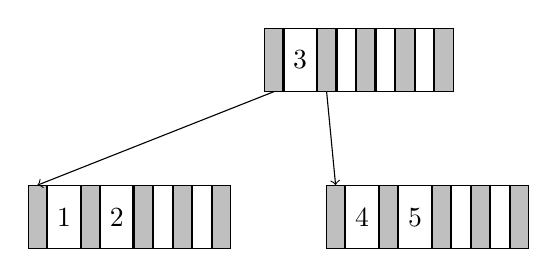
\begin{tikzpicture}[
            start chain=0 going right,
            defaultNode/.style={defaultNode1},
        ]

        %Level0
		\draw pic {firstInnerNode={3}{}{}{}{0}{0}{5}};

        %Level1
        \draw pic {firstInnerNode={1}{2}{}{}{1}{1}{2}};
        \draw pic {innerNode={4}{5}{}{}{1}{2}};

        %Verbindungspfeile 0 - 1
        \draw pic {connect={0}{0}{1}};
        \draw pic {connect={0}{1}{2}};
    \end{tikzpicture}
\end{center}

6 und 7 können wieder ohne Splitt in den rechten Blattknoten eingefügt werden.

\begin{center}
    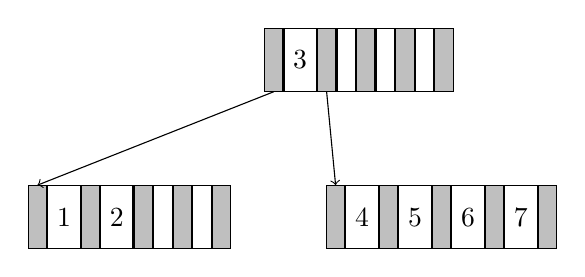
\begin{tikzpicture}[
            start chain=0 going right,
            defaultNode/.style={defaultNode1},
        ]

        %Level0
        \draw pic {firstInnerNode={3}{}{}{}{0}{0}{5}};

        %Level1
        \draw pic {firstInnerNode={1}{2}{}{}{1}{1}{2}};
        \draw pic {innerNode={4}{5}{6}{7}{1}{2}};

        %Verbindungspfeile 0 - 1
        \draw pic {connect={0}{0}{1}};
        \draw pic {connect={0}{1}{2}};
    \end{tikzpicture}
\end{center}

Das Einfügen der 8 führt zum Überlauf im rechten Blattknoten.
Der Knoten wird also an der 6 gesplittet, die in den Wurzelknoten wandert:

\begin{center}
    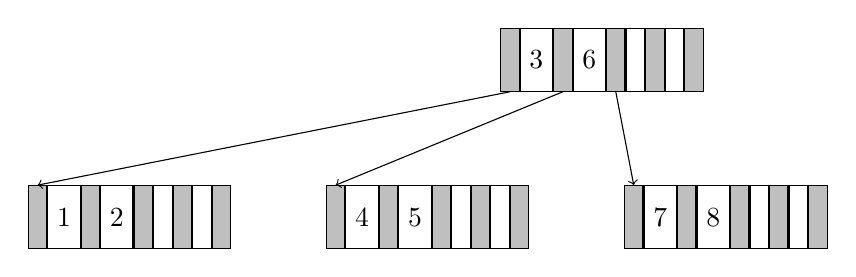
\begin{tikzpicture}[
            start chain=0 going right,
            defaultNode/.style={defaultNode1},
        ]

        %Level0
        \draw pic {firstInnerNode={3}{6}{}{}{0}{0}{8}};

        %Level1
        \draw pic {firstInnerNode={1}{2}{}{}{1}{1}{2}};
        \draw pic {innerNode={4}{5}{}{}{1}{2}};
        \draw pic {innerNode={7}{8}{}{}{1}{3}};

        %Verbindungspfeile 0 - 1
        \draw pic {connect={0}{0}{1}};
        \draw pic {connect={0}{1}{2}};
        \draw pic {connect={0}{2}{3}};
    \end{tikzpicture}
\end{center}

9 und 10 können wieder ohne Splitt eingefügt werden.
Beim Einfügen der 11 wird der rechte Blattknoten wieder gesplittet,
9 wird in den Wurzelknoten gezogen.
Das gleiche gilt für das Einfügen von 12, 13 und 14, nun ist der Wurzelknoten voll:

\begin{center}
    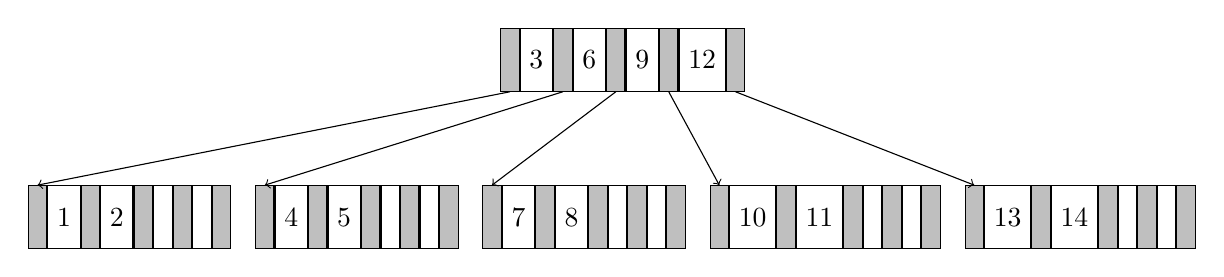
\begin{tikzpicture}[
            start chain=0 going right,
            defaultNode/.style={defaultNode2},
        ]

        %Level0
        \draw pic {firstInnerNode={3}{6}{9}{12}{0}{0}{8}};

        %Level1
        \draw pic {firstInnerNode={1}{2}{}{}{1}{1}{2}};
        \draw pic {innerNodeNarrow={4}{5}{}{}{1}{2}};
        \draw pic {innerNodeNarrow={7}{8}{}{}{1}{3}};
        \draw pic {innerNodeNarrow={10}{11}{}{}{1}{4}};
        \draw pic {innerNodeNarrow={13}{14}{}{}{1}{5}};

        %Verbindungspfeile 0 - 1
        \draw pic {connect={0}{0}{1}};
        \draw pic {connect={0}{1}{2}};
        \draw pic {connect={0}{2}{3}};
        \draw pic {connect={0}{3}{4}};
        \draw pic {connect={0}{4}{5}};
    \end{tikzpicture}
\end{center}

15 und 16 können wieder einfach in den rechten Blattknoten eingefügt werden.
Das Einfügen der 17 führt zum Splitt im rechten Blattknoten.
Da der Wurzelknoten aber bereits voll ist, führt das auch zum Wurzelsplitt.
Der entstehende Baum sieht dann so aus:

\begin{center}
    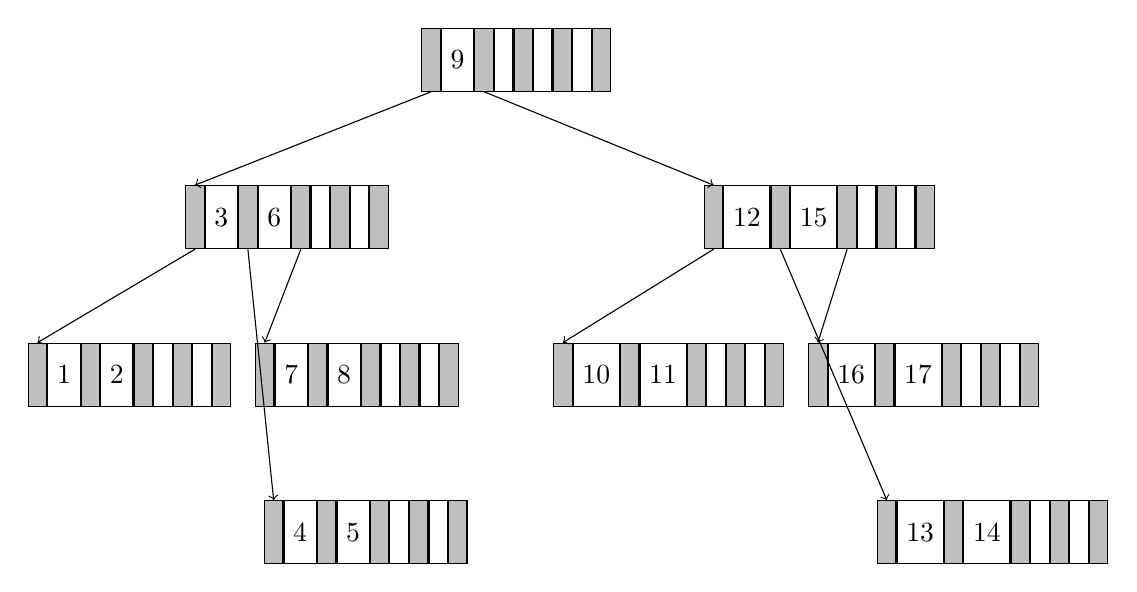
\begin{tikzpicture}[
            start chain=0 going right,
            defaultNode/.style={defaultNode2},
        ]

        %Level0
        \draw pic {firstInnerNode={9}{}{}{}{0}{0}{5}};

        %Level1
        \draw pic {firstInnerNode={3}{6}{}{}{1}{1}{2}};
        \draw pic {innerNodeVar={12}{15}{}{}{1}{2}{4}};

        %Level2
        \draw pic {firstInnerNode={1}{2}{}{}{2}{3}{0}};
        \draw pic {innerNodeNarrow={7}{8}{}{}{2}{5}};
        \draw pic {innerNode={10}{11}{}{}{2}{6}};
        \draw pic {innerNodeNarrow={16}{17}{}{}{2}{8}};

        %Level2.5
        \draw pic {firstInnerNode={4}{5}{}{}{3}{4}{3}};
        \draw pic {innerNodeVar={13}{14}{}{}{2}{7}{5.2}};


        %Verbindungspfeile
        \draw pic {connect={0}{0}{1}};
        \draw pic {connect={0}{1}{2}};
        \draw pic {connect={1}{0}{3}};
        \draw pic {connect={1}{1}{4}};
        \draw pic {connect={1}{2}{5}};
        \draw pic {connect={2}{0}{6}};
        \draw pic {connect={2}{1}{7}};
        \draw pic {connect={2}{2}{8}};
    \end{tikzpicture}
\end{center}

18 und 19 lassen sich nun wieder einfach in den letzten Blattknoten einfügen,
bei der 20 kommt es erneut zu einem Überlauf und einem Splitt.

Am Ende erhält man folgenden B-Baum:

\begin{center}
    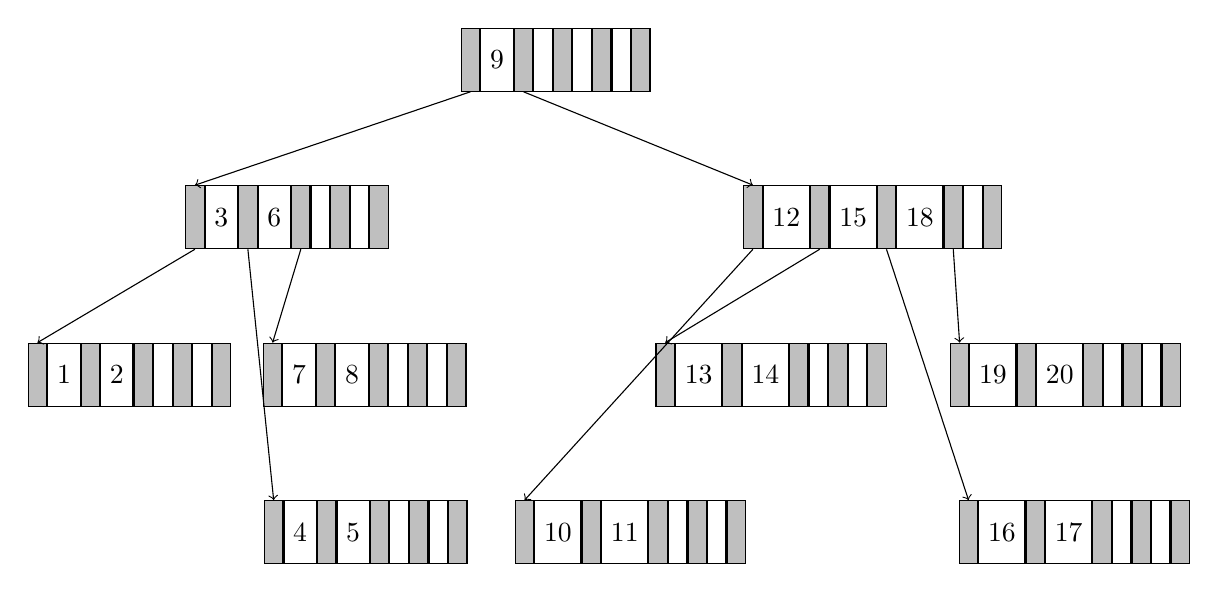
\begin{tikzpicture}[
            start chain=0 going right,
            defaultNode/.style={defaultNode2},
        ]

        %Level0
        \draw pic {firstInnerNode={9}{}{}{}{0}{0}{6}};

        %Level1
        \draw pic {firstInnerNode={3}{6}{}{}{1}{1}{2.5}};
        \draw pic {innerNodeVar={12}{15}{18}{}{1}{2}{4.5}};

        %Level2
        \draw pic {firstInnerNode={1}{2}{}{}{2}{3}{0.5}};
        \draw pic {innerNodeVar={7}{8}{}{}{2}{5}{0.4}};
        \draw pic {innerNodeVar={13}{14}{}{}{2}{7}{2.4}};
        \draw pic {innerNodeVar={19}{20}{}{}{2}{9}{0.8}};

        %Level2.5
        \draw pic {firstInnerNode={4}{5}{}{}{3}{4}{3.5}};
        \draw pic {innerNodeVar={10}{11}{}{}{3}{6}{0.6}};
        \draw pic {innerNodeVar={16}{17}{}{}{3}{8}{2.7}};


        %Verbindungspfeile
        \draw pic {connect={0}{0}{1}};
        \draw pic {connect={0}{1}{2}};
        \draw pic {connect={1}{0}{3}};
        \draw pic {connect={1}{1}{4}};
        \draw pic {connect={1}{2}{5}};
        \draw pic {connect={2}{0}{6}};
        \draw pic {connect={2}{1}{7}};
        \draw pic {connect={2}{2}{8}};
        \draw pic {connect={2}{3}{9}};
    \end{tikzpicture}
\end{center}

Es fällt auf, dass der B-Baum nahezu minimale Auslastung aufweist. Dies liegt am sequentiellen Einfügen einer aufsteigenden Zahlenfolge in den B-Baum: Nach dem Aufspalten eines Knotens werden in den Knoten, der die kleineren Datensätze enthält, keine weiteren Werte mehr eingefügt.

Es fällt außerdem auf, dass in der Wurzelebene und in den inneren Ebenen jeweils immer nur Vielfache einer bestimmten Zahl $x$ auftreten. Bei genauerem Betrachten findet man heraus, dass sich diese Zahl $x$ für jede Ebene $i$ folgendermaßen berechnen lässt:
\[x = (k + 1)^{h - i}, i \in \mathbb{N}_{>0},\; h: \mathrm{H"ohe\ des\ Baums}\]

Erläuterung:
\begin{enumerate}[\arabic{enumii}.]
\item Wir stellen fest, dass alle „linken Kindblöcke“ durch das Splitten in unserem Beispiel immer zwei (also $k$) Elemente pro Block beinhalten.
\item Der linke Unterbaum besitzt in der ersten Ebene als Wurzel einen Knoten, welcher in der Ebene unter unserer betrachteten Ebene liegt.
Somit beinhaltet dieser zwei Elemente und drei Nachfolgeknoten, es sei denn, es handelt sich um einen Blattknoten.
\item Jeder dieser drei Nachfolger in der zweiten Ebene beinhaltet wieder zwei Elemente und hat damit drei Nachfolger, wenn es sich nicht um einen Blattknoten handelt.
Damit befinden sich in der dritten Ebene $3^2 = 9$ Knoten.
\item Führt man nun die Reihe fort kommt man mit der Unterbaumhöhe u auf die folgende Formel für die Anzahl der Elemente des linken Unterbaums:
\[(1 + 3 +3^2 +3^3 \ldots + 3^{u-1}) \cdot 2\]
\item Durch $u:= h-i$ mit h als Gesamthöhe und i als Ebene des betrachteten Knotens ergibt sich folgende allgemeine Summe:
\[(1 + (k+1) + (k+1)^2 + (k+1)^3 + \ldots + (k+1)^{h-i-1}) \cdot k = \left(\sum_{j=0}^{h-i-1} (k+1)^j\right)\cdot k \]
\item Das "`linkeste Element"' in unserer betrachteten Ebene ist damit dann das nächstgrößere Element, was sich mithilfe der geometrischen Reihe ($\sum_{i=0}^{n-1}q^i = \frac{q^n - 1}{q - 1}$) folgendermaßen berechnen lässt:
\begin{align*}
Wert &:= \text{Elemente im Unterbaum} + 1\\
& = \left(\sum_{j=0}^{h-i-1} (k+1)^j\right)\cdot k +1 \stackrel{\text{Geometrische Reihe}}{=} \frac{(k+1)^{h-i}-1}{k + 1 - 1}\cdot k + 1\\
&= (k+1)^{h-i}- 1 +1 = (k+1)^{h-i}
\end{align*}
\item Zwischen diesem "`linkesten Element"' und dem nächsten Element der Ebene befindet sich nun wieder ein Unterbaum, welcher die selbe Höhe wie der erste Unterbaum besitzt.
Damit enthält dieser wieder $(k+1)^{h-i} - 1$ Elemente und somit lautet der Wert des Elements $2\cdot (k+1)^{h-i}$.
\item Somit befinden sich in einer Ebene nur Vielfache des "`linkesten Elements"'.
\end{enumerate}
\end{solution}

\item Löschen Sie nun den Eintrag 9 und zeichnen Sie den entstehenden Baum.

\begin{solution}
Da ein innerer Eintrag gelöscht wird, muss er durch den direkten Vorgänger oder Nachfolger ersetzt werden.
Da Vorgänger- und Nachfolgerblattknoten gleich viele Einträge haben, können wir uns frei zwischen Vorgänger und Nachfolger entscheiden. Wir nehmen hier den Vorgänger 8:

\begin{note}
	Wir nehmen die 8, weil die 10 einfacher ist, da im rechten Teilbaum die 18 exisitiert, und so kein Wurzel-merge n\"otig ist.
\end{note}

\begin{center}
    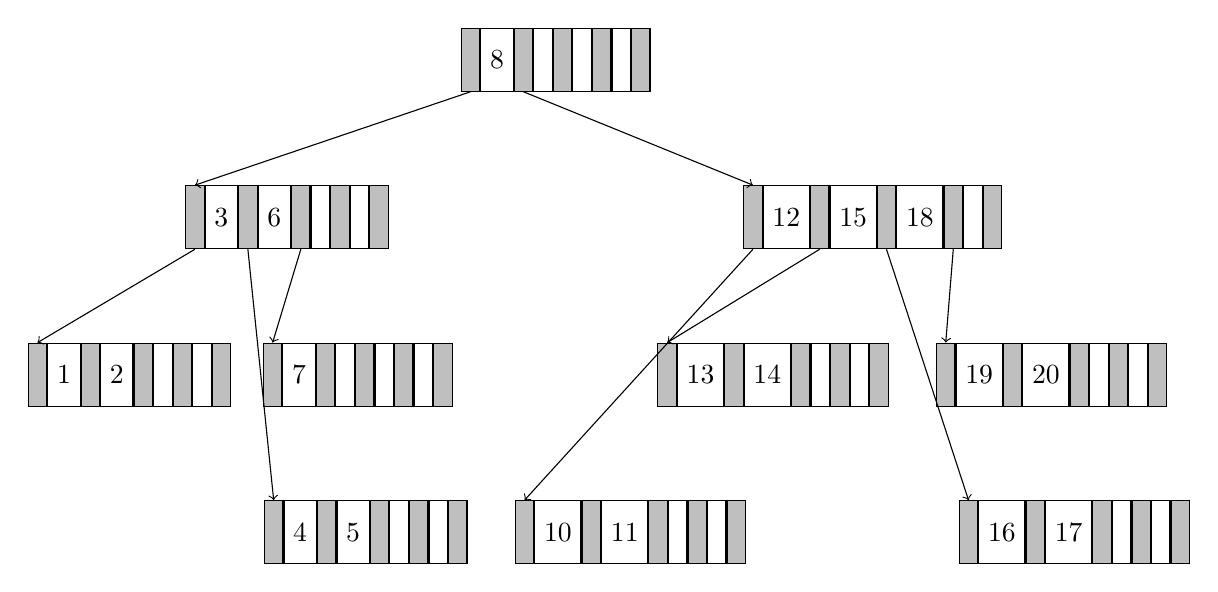
\begin{tikzpicture}[
            start chain=0 going right,
            defaultNode/.style={defaultNode2},
        ]

        %Level0
        \draw pic {firstInnerNode={8}{}{}{}{0}{0}{6}};

        %Level1
        \draw pic {firstInnerNode={3}{6}{}{}{1}{1}{2.5}};
        \draw pic {innerNodeVar={12}{15}{18}{}{1}{2}{4.5}};

        %Level2
        \draw pic {firstInnerNode={1}{2}{}{}{2}{3}{0.5}};
        \draw pic {innerNodeVar={7}{}{}{}{2}{5}{0.4}};
        \draw pic {innerNodeVar={13}{14}{}{}{2}{7}{2.6}};
        \draw pic {innerNodeVar={19}{20}{}{}{2}{9}{0.6}};

        %Level2.5
        \draw pic {firstInnerNode={4}{5}{}{}{3}{4}{3.5}};
        \draw pic {innerNodeVar={10}{11}{}{}{3}{6}{0.6}};
        \draw pic {innerNodeVar={16}{17}{}{}{3}{8}{2.7}};


        %Verbindungspfeile
        \draw pic {connect={0}{0}{1}};
        \draw pic {connect={0}{1}{2}};
        \draw pic {connect={1}{0}{3}};
        \draw pic {connect={1}{1}{4}};
        \draw pic {connect={1}{2}{5}};
        \draw pic {connect={2}{0}{6}};
        \draw pic {connect={2}{1}{7}};
        \draw pic {connect={2}{2}{8}};
        \draw pic {connect={2}{3}{9}};
    \end{tikzpicture}
\end{center}


Dadurch entsteht ein Unterlauf im Blattknoten,
der deshalb mit dem Elternknoten gemischt werden muss:

\begin{center}
    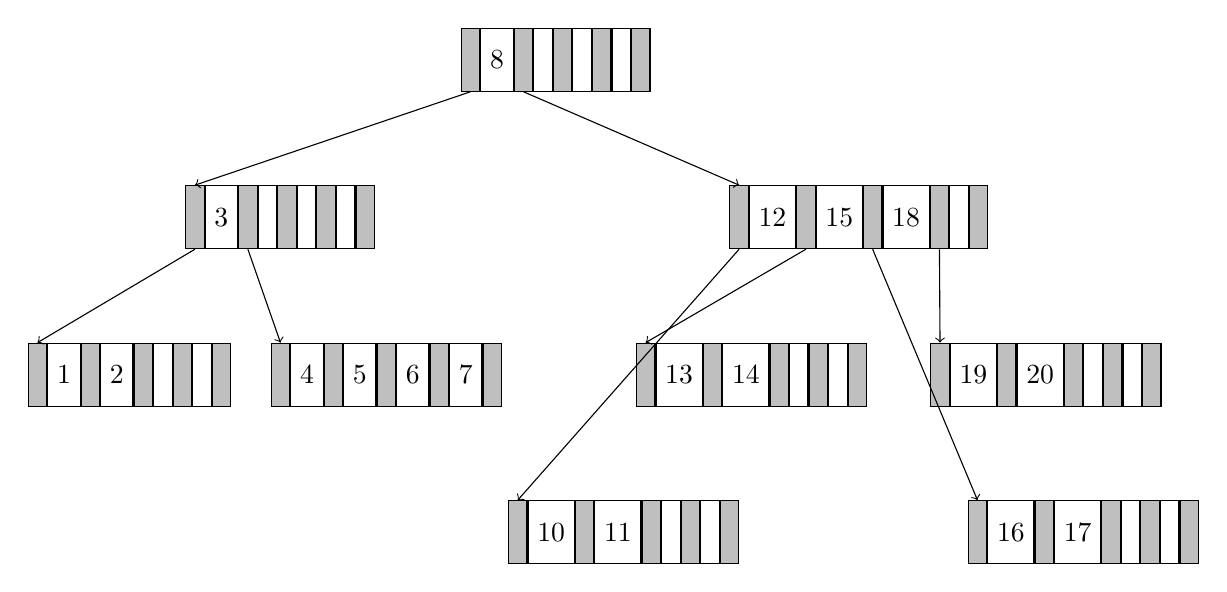
\begin{tikzpicture}[
            start chain=0 going right,
            defaultNode/.style={defaultNode2},
        ]

        %Level0
        \draw pic {firstInnerNode={8}{}{}{}{0}{0}{6}};

        %Level1
        \draw pic {firstInnerNode={3}{}{}{}{1}{1}{2.5}};
        \draw pic {innerNodeVar={12}{15}{18}{}{1}{2}{4.5}};

        %Level2
        \draw pic {firstInnerNode={1}{2}{}{}{2}{3}{0.5}};
        \draw pic {innerNodeVar={4}{5}{6}{7}{3}{4}{0.5}};
        \draw pic {innerNodeVar={13}{14}{}{}{2}{7}{1.7}};
        \draw pic {innerNodeVar={19}{20}{}{}{2}{9}{0.8}};

        %Level2.5
        \draw pic {firstInnerNode={10}{11}{}{}{3}{6}{6.6}};
        \draw pic {innerNodeVar={16}{17}{}{}{3}{8}{2.9}};


        %Verbindungspfeile
        \draw pic {connect={0}{0}{1}};
        \draw pic {connect={0}{1}{2}};
        \draw pic {connect={1}{0}{3}};
        \draw pic {connect={1}{1}{4}};
        \draw pic {connect={2}{0}{6}};
        \draw pic {connect={2}{1}{7}};
        \draw pic {connect={2}{2}{8}};
        \draw pic {connect={2}{3}{9}};
    \end{tikzpicture}
\end{center}

Nun besteht aber im linken inneren Knoten ein Unterlauf, der aufgelöst werden muss.
Dazu wird mit der Wurzel gemischt. Es entsteht ein Überlauf in der (neuen) Wurzel,
die deshalb gesplittet werden muss. Ergebnis:

\begin{center}
    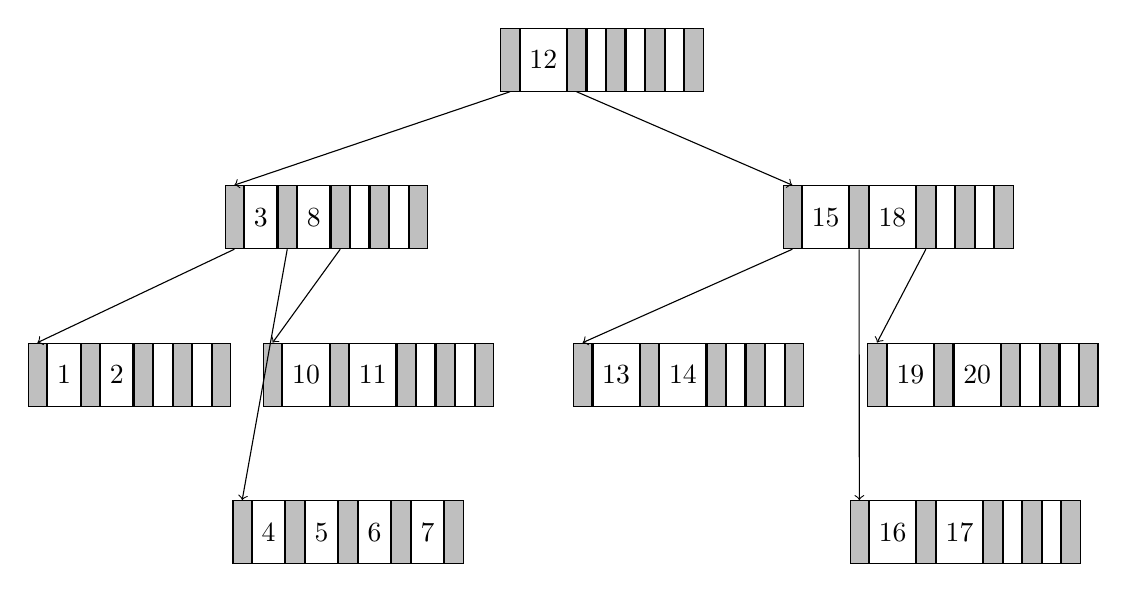
\begin{tikzpicture}[
            start chain=0 going right,
            defaultNode/.style={defaultNode2},
        ]

        %Level0
        \draw pic {firstInnerNode={12}{}{}{}{0}{0}{6}};

        %Level1
        \draw pic {firstInnerNode={3}{8}{}{}{1}{1}{2.5}};
        \draw pic {innerNodeVar={15}{18}{}{}{1}{2}{4.5}};

        %Level2
        \draw pic {firstInnerNode={1}{2}{}{}{2}{3}{0}};
        \draw pic {innerNodeVar={10}{11}{}{}{2}{5}{0.4}};
        \draw pic {innerNodeVar={13}{14}{}{}{2}{7}{1}};
        \draw pic {innerNodeVar={19}{20}{}{}{2}{9}{0.8}};

        %Level2.5
        \draw pic {firstInnerNode={4}{5}{6}{7}{3}{4}{2.6}};
        \draw pic {innerNodeVar={16}{17}{}{}{3}{8}{4.9}};


        %Verbindungspfeile
        \draw pic {connect={0}{0}{1}};
        \draw pic {connect={0}{1}{2}};
        \draw pic {connect={1}{0}{3}};
        \draw pic {connect={1}{1}{4}};
        \draw pic {connect={1}{2}{5}};
        \draw pic {connect={2}{0}{7}};
        \draw pic {connect={2}{1}{8}};
        \draw pic {connect={2}{2}{9}};
    \end{tikzpicture}
\end{center}

\end{solution}

\end{enumerate}


\begin{deeper}
\section{B-Baum die Zweite}
Fügen Sie nun die folgenden 20 Zahlen in der vorgegebenen Reihenfolge in einen leeren B-Baum mit \( k=2 \) ein:\\
3, 14, 15, 92, 65, 35, 89, 79, 32, 38, 46, 26, 43, 50, 28, 84, 19, 71, 69, 39

\begin{note}
	Die Zahlen 3, 14, 15, 92 lassen sich problemlos in den Wurzelknoten einfügen.
	\begin{center}
		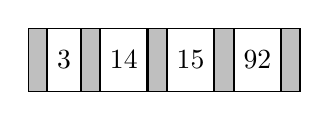
\begin{tikzpicture}[
		start chain=0 going right,
		defaultNode/.style={defaultNode1},
		]

		%Level0
		\draw pic {firstInnerNode={3}{14}{15}{92}{0}{0}{2}};
		\end{tikzpicture}
	\end{center}

Bei 65 kommt es zum Wurzelsplitt und der Baum wächst um eins.
Danach stehen 15 in der Wurzel, 3 und 14 im linken Blattknoten und 65 und 92 im rechten Blattknoten.

	\begin{center}
		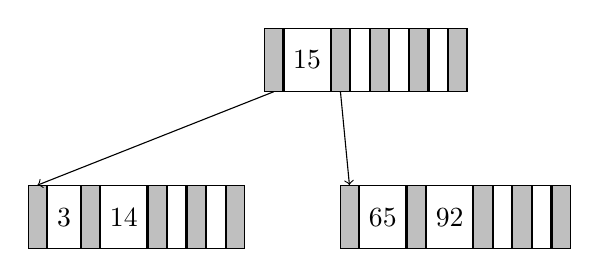
\begin{tikzpicture}[
		start chain=0 going right,
		defaultNode/.style={defaultNode1},
		]

		%Level0
		\draw pic {firstInnerNode={15}{}{}{}{0}{0}{5}};

		%Level1
		\draw pic {firstInnerNode={3}{14}{}{}{1}{1}{2}};
		\draw pic {innerNode={65}{92}{}{}{1}{2}};

		%Verbindungspfeile 0 - 1
		\draw pic {connect={0}{0}{1}};
		\draw pic {connect={0}{1}{2}};
		\end{tikzpicture}
	\end{center}

35 und 89 können wieder ohne Splitt in den rechten Blattknoten eingefügt werden, bis es dann bei der 79 zu einem Splitt kommt.

	\begin{center}
		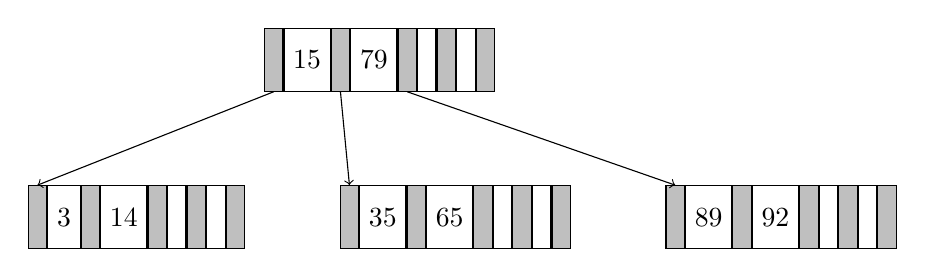
\begin{tikzpicture}[
		start chain=0 going right,
		defaultNode/.style={defaultNode1},
		]

		%Level0
		\draw pic {firstInnerNode={15}{79}{}{}{0}{0}{5}};

		%Level1
		\draw pic {firstInnerNode={3}{14}{}{}{1}{1}{2}};
		\draw pic {innerNode={35}{65}{}{}{1}{2}};
		\draw pic {innerNode={89}{92}{}{}{1}{3}};

		%Verbindungspfeile 0 - 11
		\draw pic {connect={0}{0}{1}};
		\draw pic {connect={0}{1}{2}};
		\draw pic {connect={0}{2}{3}};
		\end{tikzpicture}
	\end{center}

32 und 38 können wieder ohne Probleme in den mittleren Blattknoten eingefügt werden. Erst bei der 46 kommt es wieder zu einem Überlauf.

	\begin{center}
		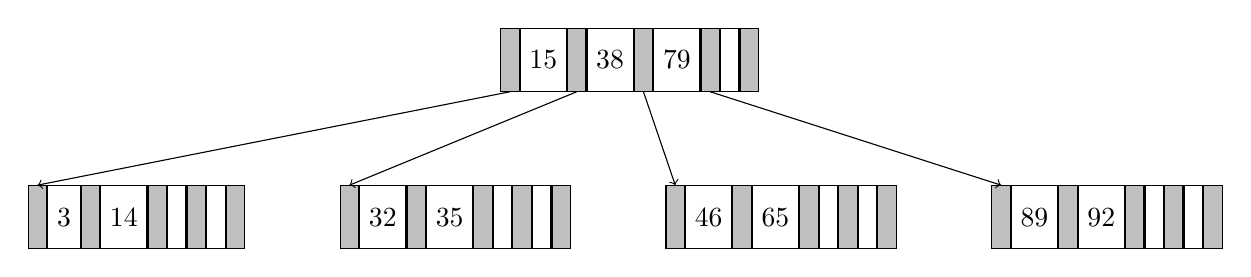
\begin{tikzpicture}[
		start chain=0 going right,
		defaultNode/.style={defaultNode1},
		]

		%Level0
		\draw pic {firstInnerNode={15}{38}{79}{}{0}{0}{8}};

		%Level1
		\draw pic {firstInnerNode={3}{14}{}{}{1}{1}{2}};
		\draw pic {innerNode={32}{35}{}{}{1}{2}};
		\draw pic {innerNode={46}{65}{}{}{1}{3}};
		\draw pic {innerNode={89}{92}{}{}{1}{4}};

		%Verbindungspfeile 0 - 1
		\draw pic {connect={0}{0}{1}};
		\draw pic {connect={0}{1}{2}};
		\draw pic {connect={0}{2}{3}};
		\draw pic {connect={0}{3}{4}};
		\end{tikzpicture}
	\end{center}

	26, 43, 50, 28 und 84 können wieder ohne Splitt eingefügt werden.
	Beim Einfügen der 19 wird der zweite Blattknoten gesplittet,
	28 wird in den Wurzelknoten gezogen.

	\begin{center}
		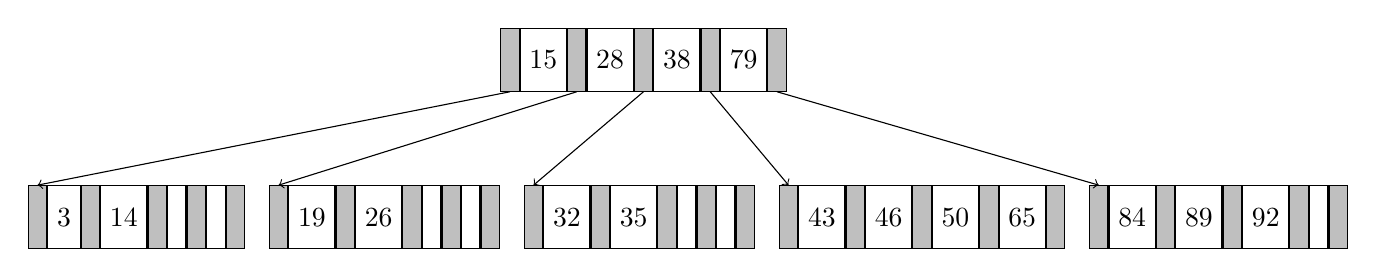
\begin{tikzpicture}[
		start chain=0 going right,
		defaultNode/.style={defaultNode2},
		]

		%Level0
		\draw pic {firstInnerNode={15}{28}{38}{79}{0}{0}{8}};

		%Level1
		\draw pic {firstInnerNode={3}{14}{}{}{1}{1}{2}};
		\draw pic {innerNodeNarrow={19}{26}{}{}{1}{2}};
		\draw pic {innerNodeNarrow={32}{35}{}{}{1}{3}};
		\draw pic {innerNodeNarrow={43}{46}{50}{65}{1}{4}};
		\draw pic {innerNodeNarrow={84}{89}{92}{}{1}{5}};

		%Verbindungspfeile 0 - 1
		\draw pic {connect={0}{0}{1}};
		\draw pic {connect={0}{1}{2}};
		\draw pic {connect={0}{2}{3}};
		\draw pic {connect={0}{3}{4}};
		\draw pic {connect={0}{4}{5}};
		\end{tikzpicture}
	\end{center}

Das Einfügen der 71 führt zum Splitt im Blattknoten. die 50 wird nach oben geschoben und es kommt zum Überlauf im Wurzelknoten. Dieser wird gesplittet und die 38 wandert nach oben.
Der entstehende Baum sieht dann so aus:

	\begin{center}
		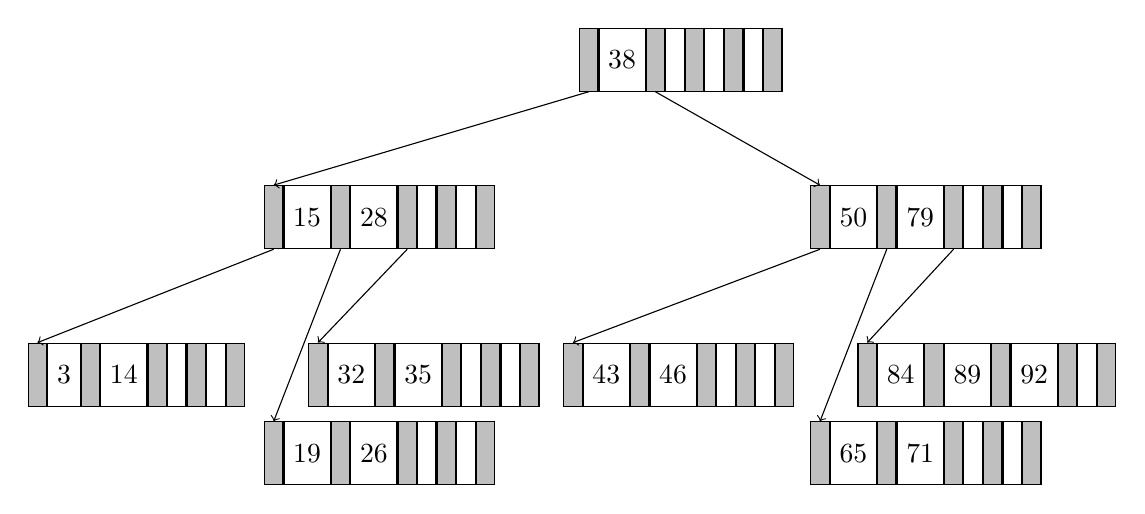
\begin{tikzpicture}[
		start chain=0 going right,
		defaultNode/.style={defaultNode2},
		]

		%Level0
		\draw pic {firstInnerNode={38}{}{}{}{0}{0}{8}};

		%Level1
		\draw pic {firstInnerNode={15}{28}{}{}{1}{1}{4}};
		\draw pic {innerNodeVar={50}{79}{}{}{1}{2}{4}};

		%Level2
		\draw pic {firstInnerNode={3}{14}{}{}{2}{3}{1}};
		\draw pic {innerNodeVar={32}{35}{}{}{2}{5}{0.8}};
		\draw pic {innerNodeNarrow={43}{46}{}{}{2}{6}};
		\draw pic {innerNodeVar={84}{89}{92}{}{2}{8}{0.8}};

		%Level2.5
		\draw pic {firstInnerNode={19}{26}{}{}{2.5}{4}{4}};
		\draw pic {innerNodeVar={65}{71}{}{}{2.5}{7}{4}};

		%Verbindungspfeile
		\draw pic {connect={0}{0}{1}};
		\draw pic {connect={0}{1}{2}};
		\draw pic {connect={1}{0}{3}};
		\draw pic {connect={1}{1}{4}};
		\draw pic {connect={1}{2}{5}};
		\draw pic {connect={2}{0}{6}};
		\draw pic {connect={2}{1}{7}};
		\draw pic {connect={2}{2}{8}};
		\end{tikzpicture}
	\end{center}

Final werden nun die 69 und 39 eingefügt.

Am Ende erhält man folgenden B-Baum:

	\begin{center}
	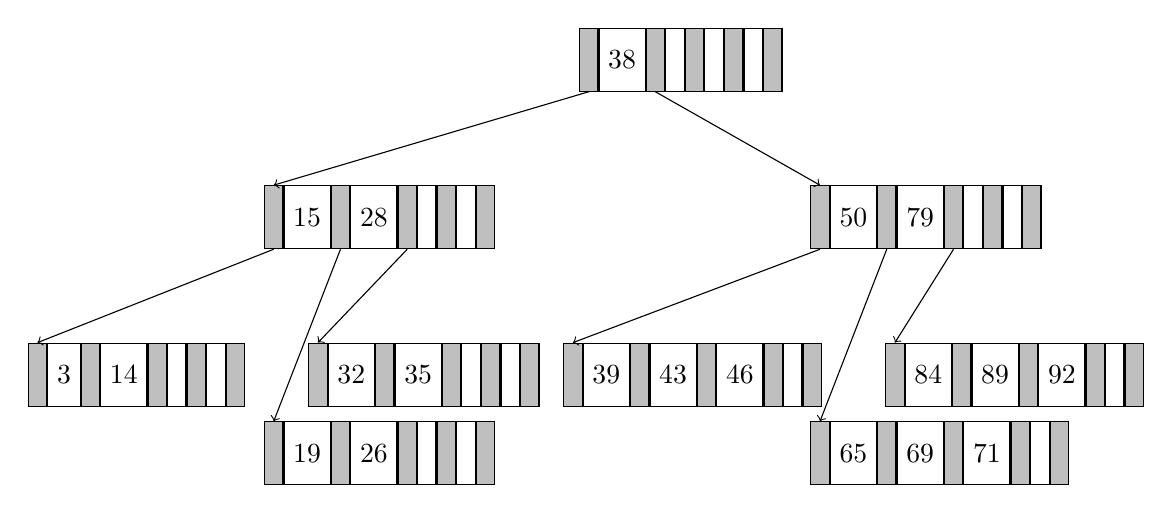
\begin{tikzpicture}[
	start chain=0 going right,
	defaultNode/.style={defaultNode2},
	]

	%Level0
	\draw pic {firstInnerNode={38}{}{}{}{0}{0}{8}};

	%Level1
	\draw pic {firstInnerNode={15}{28}{}{}{1}{1}{4}};
	\draw pic {innerNodeVar={50}{79}{}{}{1}{2}{4}};

	%Level2
	\draw pic {firstInnerNode={3}{14}{}{}{2}{3}{1}};
	\draw pic {innerNodeVar={32}{35}{}{}{2}{5}{0.8}};
	\draw pic {innerNodeNarrow={39}{43}{46}{}{2}{6}};
	\draw pic {innerNodeVar={84}{89}{92}{}{2}{8}{0.8}};

	%Level2.5
	\draw pic {firstInnerNode={19}{26}{}{}{2.5}{4}{4}};
	\draw pic {innerNodeVar={65}{69}{71}{}{2.5}{7}{4}};

	%Verbindungspfeile
	\draw pic {connect={0}{0}{1}};
	\draw pic {connect={0}{1}{2}};
	\draw pic {connect={1}{0}{3}};
	\draw pic {connect={1}{1}{4}};
	\draw pic {connect={1}{2}{5}};
	\draw pic {connect={2}{0}{6}};
	\draw pic {connect={2}{1}{7}};
	\draw pic {connect={2}{2}{8}};
	\end{tikzpicture}
\end{center}
\end{note}

\end{deeper}

\section{B*-Baum}
\label{B*}

Gegeben ist ein anfangs leerer B*-Baum. Die maximale Zahl der Einträge für einen inneren Knoten beträgt $2k$, $k = 2$. Die maximale Zahl der Einträge in einem Blattknoten beträgt $2k^*$, $k^* = 1$. Es sollen Tupel bestehend aus dem Schlüssel (einer Ganzzahl) und einem String der Länge $3$ gespeichert werden. Führen Sie die im Folgenden angegebenen Einfüge- und Löschoperationen im B*-Baum durch. Wenn sich dessen Struktur dabei ändert, zeichnen Sie den B*-Baum neu!

\begin{enumerate}[a)]
  \item Fügen Sie die folgenden Tupel in der angegeben Reihenfolge in den B*-Baum ein: \textit{(1,fan), (13,gct), (7,xxe), (8,lwc), (22,vkw), (5,wym), (2,gzw), (10,ycc)}

	\begin{solution}
Für ViseAUD: 1 fan, 13 gct, 7 xxe, 8 lwc, 22 vkw, 5 wym, 2 gzw, 10 ycc

Einfügen der Tupel mit Schlüssel 1 und 13. Der Wurzelknoten ist initial noch ein Blattknoten.

	\begin{center}
		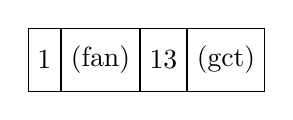
\begin{tikzpicture}[
				start chain=0 going right,
				defaultNode/.style={defaultNode1},
			]

			%Level0
			\draw pic {firstLeafNode={1}{(fan)}{13}{(gct)}{0}{0}{0}};

		\end{tikzpicture}
  \end{center}

Durch Einfügen des Tupels mit Schlüssel 7 entsteht ein Überlauf im Wurzelknoten.
Es kommt zum Splitt im Wurzelknoten.
Dadurch ist der Wurzelknoten jetzt ein innerer Knoten und es existieren zwei Blattknoten.
Der Baum wächst um eins.

	\begin{center}
		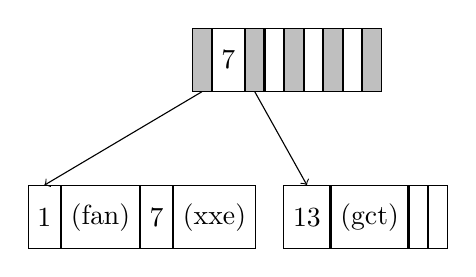
\begin{tikzpicture}[
				start chain=0 going right,
				start chain=1 going right,
				defaultNode/.style={defaultNode1},
			]

			%Level0
			\draw pic {firstInnerNode={7}{}{}{}{0}{0}{2}};

            %Level1
            \draw pic {firstLeafNode={1}{(fan)}{7}{(xxe)}{1}{1}{0}};
            \draw pic {leafNode={13}{(gct)}{}{}{1}{2}};

            %Verbindungspfeile 0 - 1
            \draw pic {connect={0}{0}{1}};
            \draw pic {connect={0}{1}{2}};

		\end{tikzpicture}
    \end{center}

Einfügen des Tupels mit Schlüssel 8.

	\begin{center}
		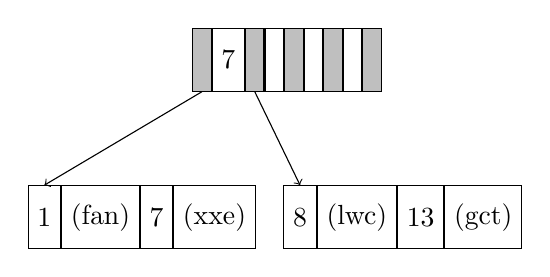
\begin{tikzpicture}[
				start chain=0 going right,
				start chain=1 going right,
				defaultNode/.style={defaultNode1},
			]

			%Level0
			\draw pic {firstInnerNode={7}{}{}{}{0}{0}{2}};

            %Level1
            \draw pic {firstLeafNode={1}{(fan)}{7}{(xxe)}{1}{1}{0}};
            \draw pic {leafNode={8}{(lwc)}{13}{(gct)}{1}{2}};

            %Verbindungspfeile 0 - 1
            \draw pic {connect={0}{0}{1}};
            \draw pic {connect={0}{1}{2}};

    \end{tikzpicture}
    \end{center}

Einfügen des Tupels mit Schlüssel 22. Im zweiten Blattknoten entsteht ein Überlauf. Es werden ein neuer Blattknoten erzeugt und im Wurzelknoten ein neuer Eintrag hinzugefügt.

	\begin{center}
		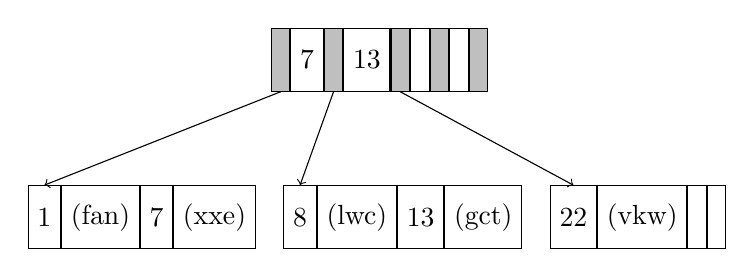
\begin{tikzpicture}[
				start chain=0 going right,
				start chain=1 going right,
				defaultNode/.style={defaultNode1},
			]

			%Level0
			\draw pic {firstInnerNode={7}{13}{}{}{0}{0}{3}};

            %Level1
            \draw pic {firstLeafNode={1}{(fan)}{7}{(xxe)}{1}{1}{0}};
            \draw pic {leafNode={8}{(lwc)}{13}{(gct)}{1}{2}};
            \draw pic {leafNode={22}{(vkw)}{}{}{1}{3}};

            %Verbindungspfeile 0 - 1
            \draw pic {connect={0}{0}{1}};
            \draw pic {connect={0}{1}{2}};
            \draw pic {connect={0}{2}{3}};

		\end{tikzpicture}
    \end{center}

Einfügen des Tupels mit Schlüssel 5. Im ersten Blattknoten entsteht ein Überlauf. Es werden ein neuer Blattknoten erzeugt und im Wurzelknoten ein neuer Eintrag hinzugefügt.

	\begin{center}
		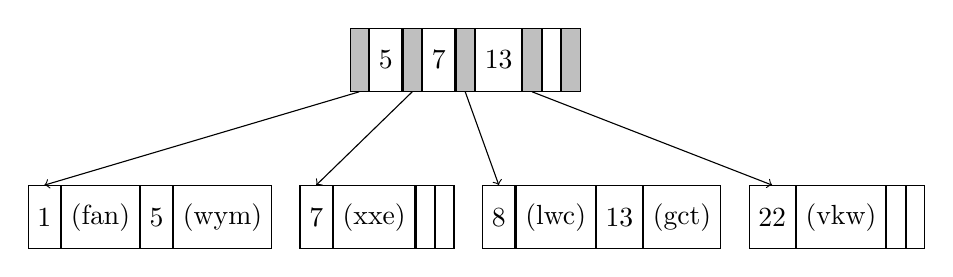
\begin{tikzpicture}[
				start chain=0 going right,
				start chain=1 going right,
				defaultNode/.style={defaultNode1},
			]

			%Level0
			\draw pic {firstInnerNode={5}{7}{13}{}{0}{0}{4}};

            %Level1
            \draw pic {firstLeafNode={1}{(fan)}{5}{(wym)}{1}{1}{0}};
            \draw pic {leafNode={7}{(xxe)}{}{}{1}{2}};
            \draw pic {leafNode={8}{(lwc)}{13}{(gct)}{1}{3}};
            \draw pic {leafNode={22}{(vkw)}{}{}{1}{4}};

            %Verbindungspfeile 0 - 1
            \draw pic {connect={0}{0}{1}};
            \draw pic {connect={0}{1}{2}};
            \draw pic {connect={0}{2}{3}};
            \draw pic {connect={0}{3}{4}};

		\end{tikzpicture}
    \end{center}

Einfügen des Tupels mit Schlüssel 2. Im ersten Blattknoten entsteht ein Überlauf. Es werden ein neuer Blattknoten erzeugt und im Wurzelknoten ein neuer Eintrag hinzugefügt.

	\begin{center}
		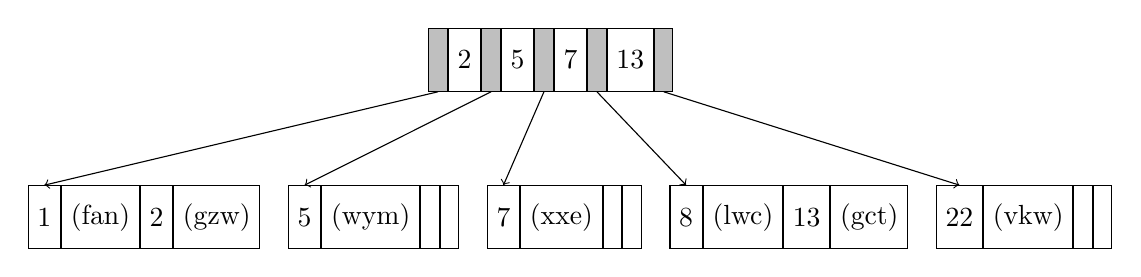
\begin{tikzpicture}[
				start chain=0 going right,
				start chain=1 going right,
				defaultNode/.style={defaultNode1},
			]

			%Level0
			\draw pic {firstInnerNode={2}{5}{7}{13}{0}{0}{5}};

            %Level1
            \draw pic {firstLeafNode={1}{(fan)}{2}{(gzw)}{1}{1}{0}};
            \draw pic {leafNode={5}{(wym)}{}{}{1}{2}};
            \draw pic {leafNode={7}{(xxe)}{}{}{1}{3}};
            \draw pic {leafNode={8}{(lwc)}{13}{(gct)}{1}{4}};
            \draw pic {leafNode={22}{(vkw)}{}{}{1}{5}};

            %Verbindungspfeile 0 - 1
            \draw pic {connect={0}{0}{1}};
            \draw pic {connect={0}{1}{2}};
            \draw pic {connect={0}{2}{3}};
            \draw pic {connect={0}{3}{4}};
            \draw pic {connect={0}{4}{5}};

		\end{tikzpicture}
    \end{center}

Einfügen des Tupels mit Schlüssel 10. Im vierten Blattknoten entsteht ein Überlauf. Es werden ein neuer Blattknoten erzeugt und im Wurzelknoten ein neuer Eintrag hinzugefügt. Es kommt zum Überlauf im Wurzelknoten. Es werden zwei neue innere Knoten erzeugt mit jeweils zwei Einträgen. Der Wurzelknoten hat einen Eintrag.

	\begin{center}
        \scalebox{0.9}{%
		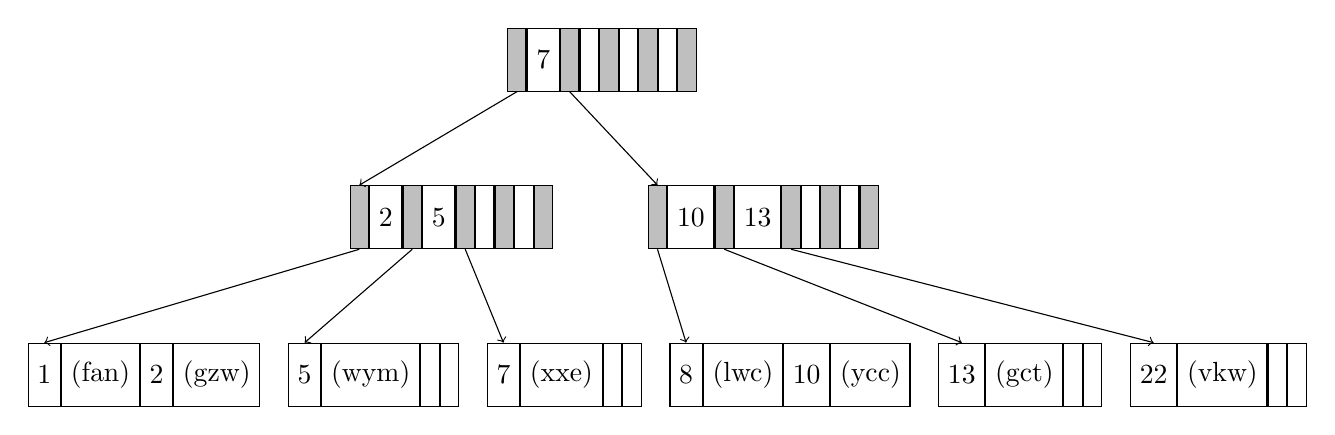
\begin{tikzpicture}[
				start chain=0 going right,
				start chain=1 going right,
				start chain=2 going right,
				defaultNode/.style={defaultNode1}
			]

			%Level0
			\draw pic {firstInnerNode={7}{}{}{}{0}{0}{6}};

			%Level1
			\draw pic {firstInnerNode={2}{5}{}{}{1}{1}{4}};
			\draw pic {innerNode={10}{13}{}{}{1}{2}};

			%Level2
			\draw pic {firstLeafNode={1}{(fan)}{2}{(gzw)}{2}{3}{0}};
			\draw pic {leafNode={5}{(wym)}{}{}{2}{4}};
			\draw pic {leafNode={7}{(xxe)}{}{}{2}{5}};
			\draw pic {leafNode={8}{(lwc)}{10}{(ycc)}{2}{6}};
			\draw pic {leafNode={13}{(gct)}{}{}{2}{7}};
			\draw pic {leafNode={22}{(vkw)}{}{}{2}{8}};

			%Verbindungspfeile
			%Level 0 -> 1
			\draw pic {connect={0}{0}{1}};
			\draw pic {connect={0}{1}{2}};
			%Level 1->2
			\draw pic {connect={1}{0}{3}};
			\draw pic {connect={1}{1}{4}};
			\draw pic {connect={1}{2}{5}};
			\draw pic {connect={2}{0}{6}};
			\draw pic {connect={2}{1}{7}};
			\draw pic {connect={2}{2}{8}};

		\end{tikzpicture}
        }
    \end{center}
	\end{solution}

	\item Löschen Sie jetzt den Datensatz mit Schlüssel $10$, danach den mit Schlüssel $13$.

	\begin{solution}
	Löschen des Tupels mit Schlüssel 10 (also $(10,ycc)$) aus dem vierten Blattknoten.\\

	\begin{center}
		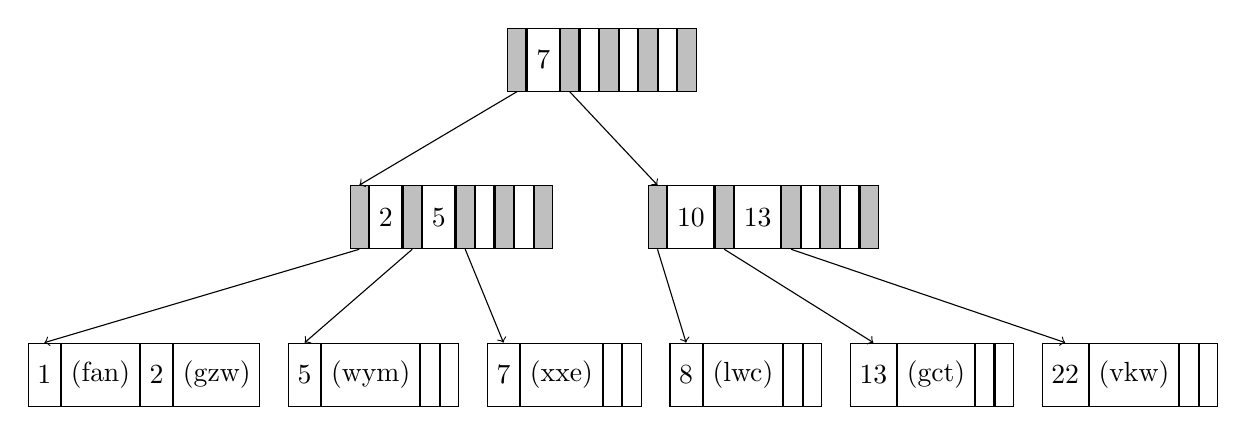
\begin{tikzpicture}[
				start chain=0 going right,
				start chain=1 going right,
				start chain=2 going right,
				defaultNode/.style={defaultNode1},
			]

			%Level0
			\draw pic {firstInnerNode={7}{}{}{}{0}{0}{6}};

			%Level1
			\draw pic {firstInnerNode={2}{5}{}{}{1}{1}{4}};
			\draw pic {innerNode={10}{13}{}{}{1}{2}};

			%Level2
			\draw pic {firstLeafNode={1}{(fan)}{2}{(gzw)}{2}{3}{0}};
			\draw pic {leafNode={5}{(wym)}{}{}{2}{4}};
			\draw pic {leafNode={7}{(xxe)}{}{}{2}{5}};
			\draw pic {leafNode={8}{(lwc)}{}{}{2}{6}};
			\draw pic {leafNode={13}{(gct)}{}{}{2}{7}};
			\draw pic {leafNode={22}{(vkw)}{}{}{2}{8}};

			%Verbindungspfeile
			%Level 0 -> 1
			\draw pic {connect={0}{0}{1}};
			\draw pic {connect={0}{1}{2}};
			%Level 1->2
			\draw pic {connect={1}{0}{3}};
			\draw pic {connect={1}{1}{4}};
			\draw pic {connect={1}{2}{5}};
			\draw pic {connect={2}{0}{6}};
			\draw pic {connect={2}{1}{7}};
			\draw pic {connect={2}{2}{8}};

		\end{tikzpicture}
    \end{center}

	Löschen von 13 führt zu Unterlauf in Blattknoten.

	\begin{center}
		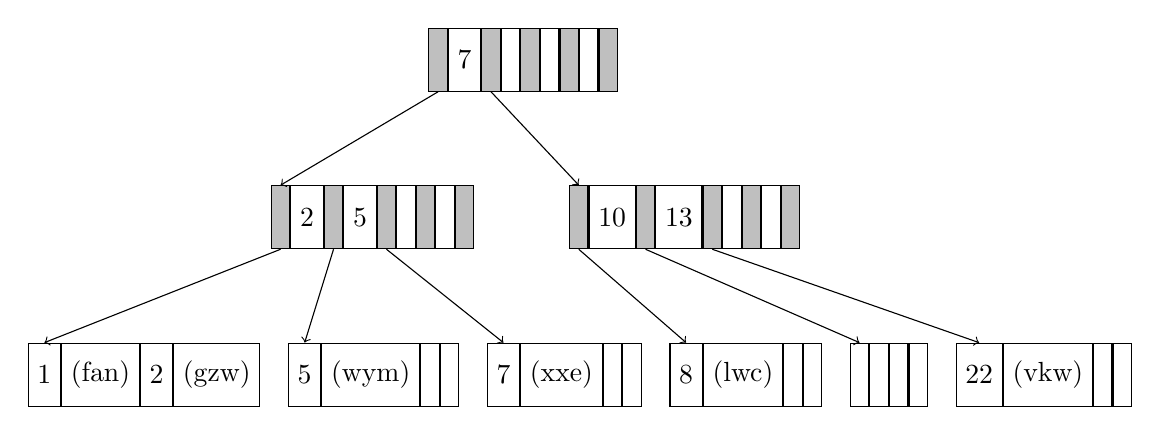
\begin{tikzpicture}[
				start chain=0 going right,
				start chain=1 going right,
				start chain=2 going right,
				defaultNode/.style={defaultNode1},
			]

			%Level0
			\draw pic {firstInnerNode={7}{}{}{}{0}{0}{5}};

			%Level1
			\draw pic {firstInnerNode={2}{5}{}{}{1}{1}{3}};
			\draw pic {innerNode={10}{13}{}{}{1}{2}};

			%Level2
			\draw pic {firstLeafNode={1}{(fan)}{2}{(gzw)}{2}{3}{0}};
			\draw pic {leafNode={5}{(wym)}{}{}{2}{4}};
			\draw pic {leafNode={7}{(xxe)}{}{}{2}{5}};
			\draw pic {leafNode={8}{(lwc)}{}{}{2}{6}};
			\draw pic {leafNode={}{}{}{}{2}{7}};
			\draw pic {leafNode={22}{(vkw)}{}{}{2}{8}};

			%Verbindungspfeile
			%Level 0 -> 1
			\draw pic {connect={0}{0}{1}};
			\draw pic {connect={0}{1}{2}};
			%Level 1->2
			\draw pic {connect={1}{0}{3}};
			\draw pic {connect={1}{1}{4}};
			\draw pic {connect={1}{2}{5}};
			\draw pic {connect={2}{0}{6}};
			\draw pic {connect={2}{1}{7}};
			\draw pic {connect={2}{2}{8}};


		\end{tikzpicture}
    \end{center}

Untergelaufenen Blattknoten mit benachbartem Knoten mischen (hier mit rechtem Nachbarknoten). Entfernen des entsprechenden Eintrags im inneren Knoten. Führt zu Unterlauf im inneren Knoten.

	\begin{center}
		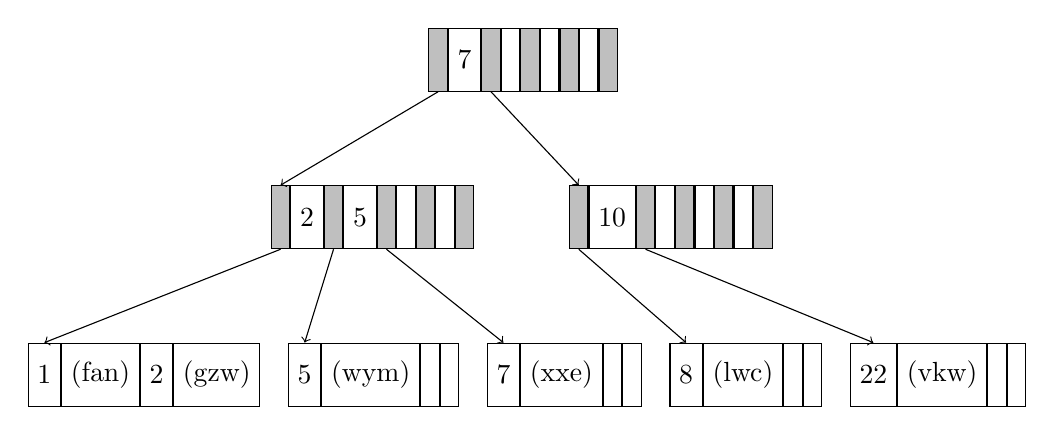
\begin{tikzpicture}[
				start chain=0 going right,
				start chain=1 going right,
				start chain=2 going right,
				defaultNode/.style={defaultNode1},
			]

			%Level0
			\draw pic {firstInnerNode={7}{}{}{}{0}{0}{5}};

			%Level1
			\draw pic {firstInnerNode={2}{5}{}{}{1}{1}{3}};
			\draw pic {innerNode={10}{}{}{}{1}{2}};

			%Level2
			\draw pic {firstLeafNode={1}{(fan)}{2}{(gzw)}{2}{3}{0}};
			\draw pic {leafNode={5}{(wym)}{}{}{2}{4}};
			\draw pic {leafNode={7}{(xxe)}{}{}{2}{5}};
			\draw pic {leafNode={8}{(lwc)}{}{}{2}{6}};
			\draw pic {leafNode={22}{(vkw)}{}{}{2}{7}};

			%Verbindungspfeile
			%Level 0 -> 1
			\draw pic {connect={0}{0}{1}};
			\draw pic {connect={0}{1}{2}};
			%Level 1->2
			\draw pic {connect={1}{0}{3}};
			\draw pic {connect={1}{1}{4}};
			\draw pic {connect={1}{2}{5}};
			\draw pic {connect={2}{0}{6}};
			\draw pic {connect={2}{1}{7}};

		\end{tikzpicture}
    \end{center}

Beide inneren Knoten mischen. Führt zu Unterlauf im Wurzelknoten. Baum schrumpft um eins.

	\begin{center}
		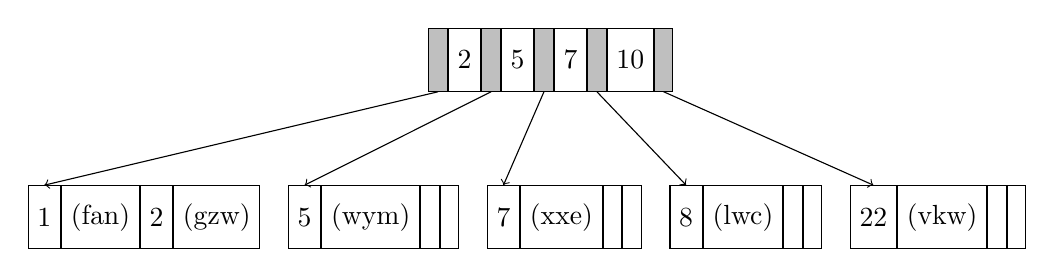
\begin{tikzpicture}[
				start chain=0 going right,
				start chain=1 going right,
				defaultNode/.style={defaultNode1},
			]

			%Level0
			\draw pic {firstInnerNode={2}{5}{7}{10}{0}{0}{5}};

            %Level1
            \draw pic {firstLeafNode={1}{(fan)}{2}{(gzw)}{1}{1}{0}};
            \draw pic {leafNode={5}{(wym)}{}{}{1}{2}};
            \draw pic {leafNode={7}{(xxe)}{}{}{1}{3}};
            \draw pic {leafNode={8}{(lwc)}{}{}{1}{4}};
            \draw pic {leafNode={22}{(vkw)}{}{}{1}{5}};

            %Verbindungspfeile 0 - 1
            \draw pic {connect={0}{0}{1}};
            \draw pic {connect={0}{1}{2}};
            \draw pic {connect={0}{2}{3}};
            \draw pic {connect={0}{3}{4}};
            \draw pic {connect={0}{4}{5}};

		\end{tikzpicture}
    \end{center}

	\end{solution}

\end{enumerate}



\begin{deeper}
\section{B*-Baum die Zweite}

Es gelten die selben Voraussetzungen wie in \ref{B*}.

\begin{enumerate}[a)]
	\item Fügen Sie die folgenden Tupel in der angegebenen Reihenfolge in den B*-Baum ein:\\
\textit{(2,wel), (71,swo), (82,st?), (13,aha), (81,hli), (8,che), (28,zah), (42,ble), (45,lda), (22,nei)
}
\begin{note}
	Einfügen der Tupel mit Schlüssel 2 und 71. Der Wurzelknoten ist initial noch ein Blattknoten.

	\begin{center}
		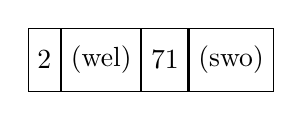
\begin{tikzpicture}[
		start chain=0 going right,
		defaultNode/.style={defaultNode1},
		]

		%Level0
		\draw pic {firstLeafNode={2}{(wel)}{71}{(swo)}{0}{0}{0}};

		\end{tikzpicture}
	\end{center}

Durch Einfügen des Tupels mit Schlüssel 82 entsteht ein Überlauf im Wurzelknoten.
Es kommt zum Splitt im Wurzelknoten.
Dadurch ist der Wurzelknoten jetzt ein innerer Knoten und es existieren zwei Blattknoten.
Der Baum wächst um eins.

	\begin{center}
		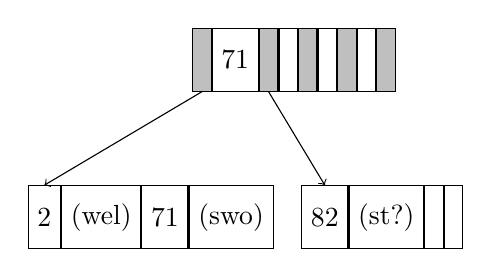
\begin{tikzpicture}[
		start chain=0 going right,
		start chain=1 going right,
		defaultNode/.style={defaultNode1},
		]

		%Level0
		\draw pic {firstInnerNode={71}{}{}{}{0}{0}{2}};

		%Level1
		\draw pic {firstLeafNode={2}{(wel)}{71}{(swo)}{1}{1}{0}};
		\draw pic {leafNode={82}{(st?)}{}{}{1}{2}};

		%Verbindungspfeile 0 - 1
		\draw pic {connect={0}{0}{1}};
		\draw pic {connect={0}{1}{2}};

		\end{tikzpicture}
	\end{center}

Das Einfügen des Tupels mit Schlüssel 13 führt wieder zu einem Überlauf und Splitt im Blattknoten.

	\begin{center}
		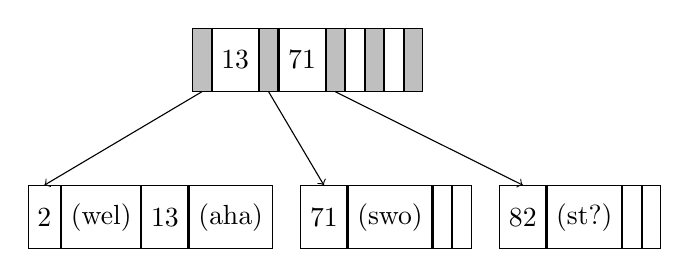
\begin{tikzpicture}[
		start chain=0 going right,
		start chain=1 going right,
		defaultNode/.style={defaultNode1},
		]

		%Level0
		\draw pic {firstInnerNode={13}{71}{}{}{0}{0}{2}};

		%Level1
		\draw pic {firstLeafNode={2}{(wel)}{13}{(aha)}{1}{1}{0}};
		\draw pic {leafNode={71}{(swo)}{}{}{1}{2}};
		\draw pic {leafNode={82}{(st?)}{}{}{1}{3}};

		%Verbindungspfeile 0 - 1
		\draw pic {connect={0}{0}{1}};
		\draw pic {connect={0}{1}{2}};
		\draw pic {connect={0}{2}{3}};
		\end{tikzpicture}
	\end{center}

Einfügen des Tupels mit Schlüssel 81.

	\begin{center}
		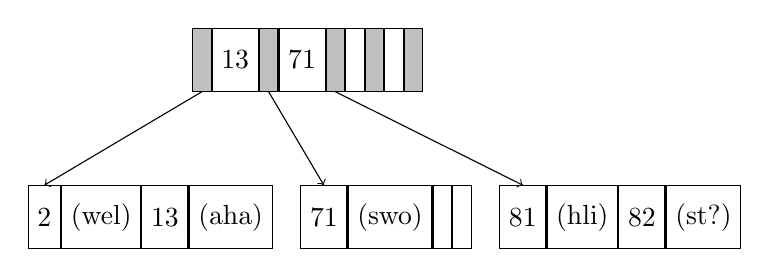
\begin{tikzpicture}[
		start chain=0 going right,
		start chain=1 going right,
		defaultNode/.style={defaultNode1},
		]

		%Level0
		\draw pic {firstInnerNode={13}{71}{}{}{0}{0}{2}};

		%Level1
		\draw pic {firstLeafNode={2}{(wel)}{13}{(aha)}{1}{1}{0}};
		\draw pic {leafNode={71}{(swo)}{}{}{1}{2}};
		\draw pic {leafNode={81}{(hli)}{82}{(st?)}{1}{3}};

		%Verbindungspfeile 0 - 1
		\draw pic {connect={0}{0}{1}};
		\draw pic {connect={0}{1}{2}};
		\draw pic {connect={0}{2}{3}};

		\end{tikzpicture}
	\end{center}

Einfügen des Tupels mit Schlüssel 8. Im ersten Blattknoten entsteht ein Überlauf. Es werden ein neuer Blattknoten erzeugt und im Wurzelknoten ein neuer Eintrag hinzugefügt.

	\begin{center}
		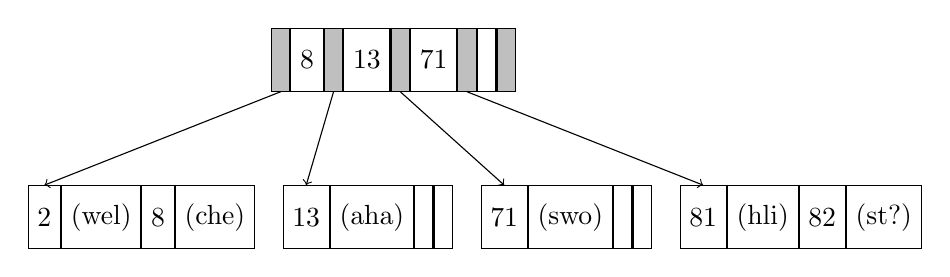
\begin{tikzpicture}[
		start chain=0 going right,
		start chain=1 going right,
		defaultNode/.style={defaultNode1},
		]

		%Level0
		\draw pic {firstInnerNode={8}{13}{71}{}{0}{0}{3}};

		%Level1
		\draw pic {firstLeafNode={2}{(wel)}{8}{(che)}{1}{1}{0}};
		\draw pic {leafNode={13}{(aha)}{}{}{1}{2}};
		\draw pic {leafNode={71}{(swo)}{}{}{1}{3}};
		\draw pic {leafNode={81}{(hli)}{82}{(st?)}{1}{4}};

		%Verbindungspfeile 0 - 1
		\draw pic {connect={0}{0}{1}};
		\draw pic {connect={0}{1}{2}};
		\draw pic {connect={0}{2}{3}};
		\draw pic {connect={0}{3}{4}};

		\end{tikzpicture}
	\end{center}

Das Einfügen des Tupels mit Schlüssel 28 verläuft ohne Überläufe. Beim Einfügen der 42 kommt es aber wieder zu einem Überlauf. Es werden ein neuer Blattknoten erzeugt und im Wurzelknoten ein neuer Eintrag hinzugefügt.

Das Einfügen der 45 verläuft nun wieder ohne Probleme.

	\begin{center}
		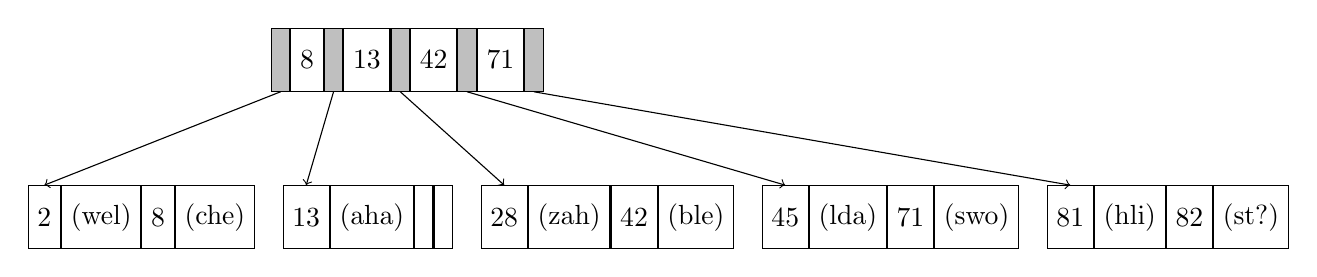
\begin{tikzpicture}[
		start chain=0 going right,
		start chain=1 going right,
		defaultNode/.style={defaultNode1},
		]

		%Level0
		\draw pic {firstInnerNode={8}{13}{42}{71}{0}{0}{3}};

		%Level1
		\draw pic {firstLeafNode={2}{(wel)}{8}{(che)}{1}{1}{0}};
		\draw pic {leafNode={13}{(aha)}{}{}{1}{2}};
		\draw pic {leafNode={28}{(zah)}{42}{(ble)}{1}{3}};
		\draw pic {leafNode={45}{(lda)}{71}{(swo)}{1}{4}};
		\draw pic {leafNode={81}{(hli)}{82}{(st?)}{1}{5}};

		%Verbindungspfeile 0 - 1
		\draw pic {connect={0}{0}{1}};
		\draw pic {connect={0}{1}{2}};
		\draw pic {connect={0}{2}{3}};
		\draw pic {connect={0}{3}{4}};
		\draw pic {connect={0}{4}{5}};

		\end{tikzpicture}
	\end{center}

Das Einfügen der 22 erzeugt nun einen Überlauf im Blattknoten und darauf im Wurzelknoten.

	\begin{center}
		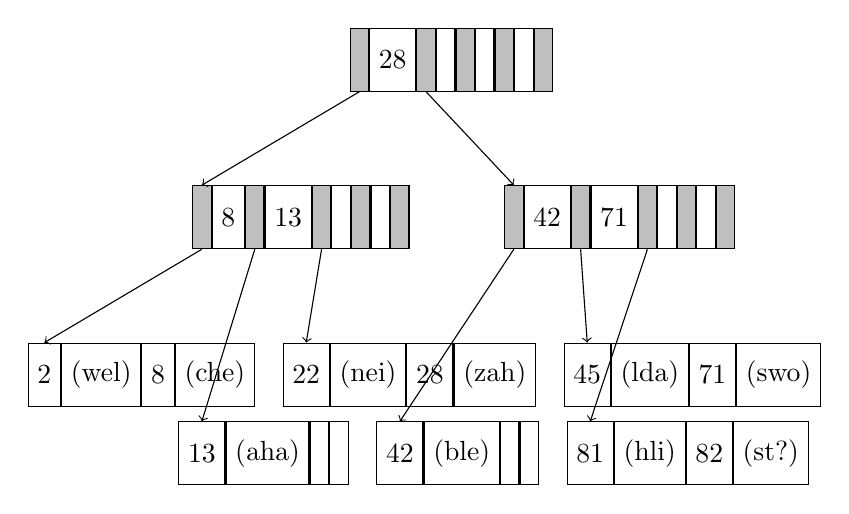
\begin{tikzpicture}[
		start chain=0 going right,
		start chain=1 going right,
		defaultNode/.style={defaultNode1},
		]

		%Level0
		\draw pic {firstInnerNode={28}{}{}{}{0}{-2}{5}};

		%level1
		\draw pic {firstInnerNode={8}{13}{}{}{1}{-1}{3}};
		\draw pic {innerNode={42}{71}{}{}{3}{0}};

		%Level2
		\draw pic {firstLeafNode={2}{(wel)}{8}{(che)}{2}{1}{1}};
		\draw pic {leafNode={22}{(nei)}{28}{(zah)}{2}{3}};
		\draw pic {leafNode={45}{(lda)}{71}{(swo)}{7}{5}};


		%Level 2.5
		\draw pic {firstLeafNode={13}{(aha)}{}{}{2.5}{2}{3}};
		\draw pic {leafNode={42}{(ble)}{}{}{2}{4}};
		\draw pic {leafNode={81}{(hli)}{82}{(st?)}{2}{6}};


		%Verbindungspfeile 0-1
		\draw pic {connect={-2}{0}{-1}};
		\draw pic {connect={-2}{1}{0}};

		%Verbindungspfeile 1 - 2
		\draw pic {connect={-1}{0}{1}};
		\draw pic {connect={-1}{1}{2}};
		\draw pic {connect={-1}{2}{3}};
		\draw pic {connect={0}{0}{4}};
		\draw pic {connect={0}{1}{5}};
		\draw pic {connect={0}{2}{6}};

		\end{tikzpicture}
	\end{center}
\end{note}

\item Löschen Sie nun die Tupel mit Schlüssel 13, 22 und 42.

Was ergibt die Zeichenkette, wenn man alle Blätter von links nach rechts liest?

\begin{note}
Löschen der 13: Unterlauf, mischen mit rechtem Knoten. Unterlauf im inneren Knoten, Mischen mit rechtem und Wurzelknoten.

	\begin{center}
		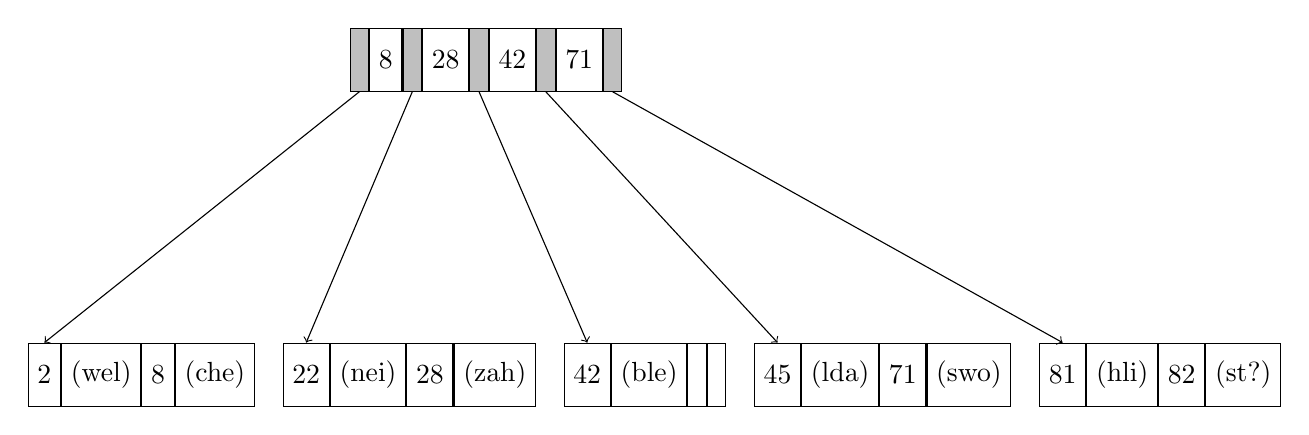
\begin{tikzpicture}[
		start chain=0 going right,
		start chain=1 going right,
		defaultNode/.style={defaultNode1},
		]

		%Level0
		\draw pic {firstInnerNode={8}{28}{42}{71}{0}{0}{5}};

		%level1
		\draw pic {firstLeafNode={2}{(wel)}{8}{(che)}{2}{1}{1}};
		\draw pic {leafNode={22}{(nei)}{28}{(zah)}{2}{2}};
		\draw pic {leafNode={42}{(ble)}{}{}{2}{3}};
		\draw pic {leafNode={45}{(lda)}{71}{(swo)}{7}{4}};
		\draw pic {leafNode={81}{(hli)}{82}{(st?)}{2}{5}};


		%Verbindungspfeile 0-1

		\draw pic {connect={0}{0}{1}};
		\draw pic {connect={0}{1}{2}};
		\draw pic {connect={0}{2}{3}};
		\draw pic {connect={0}{3}{4}};
		\draw pic {connect={0}{4}{5}};

		\end{tikzpicture}
	\end{center}

Das Löschen der 22 stellt kein Problem dar.

Beim Löschen der 42 tritt wieder ein Unterlauf mit Mischen mit dem rechten Knoten auf.

	\begin{center}
		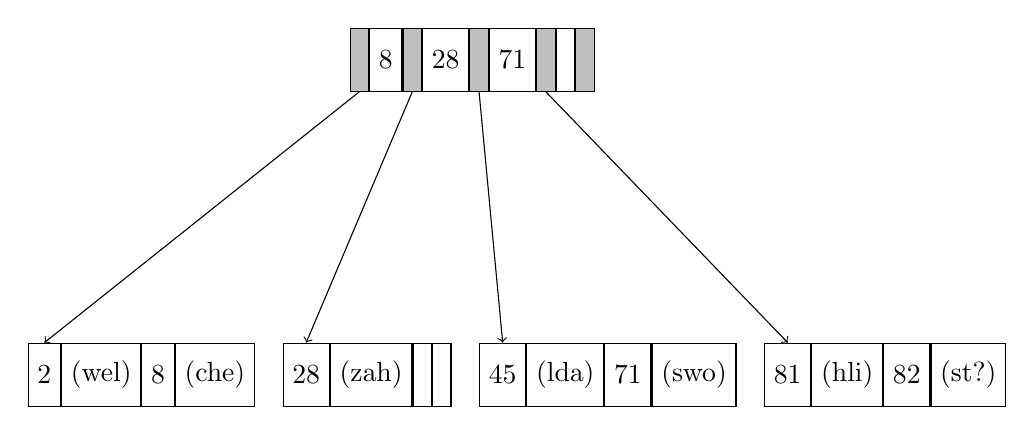
\begin{tikzpicture}[
		start chain=0 going right,
		start chain=1 going right,
		defaultNode/.style={defaultNode1},
		]

		%Level0
		\draw pic {firstInnerNode={8}{28}{71}{}{0}{0}{5}};

		%level1
		\draw pic {firstLeafNode={2}{(wel)}{8}{(che)}{2}{1}{1}};
		\draw pic {leafNode={28}{(zah)}{}{}{2}{2}};
		\draw pic {leafNode={45}{(lda)}{71}{(swo)}{7}{3}};
		\draw pic {leafNode={81}{(hli)}{82}{(st?)}{2}{4}};


		%Verbindungspfeile 0-1

		\draw pic {connect={0}{0}{1}};
		\draw pic {connect={0}{1}{2}};
		\draw pic {connect={0}{2}{3}};
		\draw pic {connect={0}{3}{4}};

		\end{tikzpicture}
	\end{center}

\end{note}

\end{enumerate}

\end{deeper}

\end{document}
